\documentclass[12pt,a4paper,twoside,openright,titlepage,final]{article}
\usepackage{fontspec}
\usepackage{amsmath}
\usepackage{amsfonts}
\usepackage{amssymb}
\usepackage{makeidx}
\usepackage{graphicx}
\usepackage[hidelinks,unicode=true]{hyperref}
\usepackage[spanish,es-nodecimaldot,es-lcroman,es-tabla,es-noshorthands]{babel}
\usepackage[left=3cm,right=2cm, bottom=4cm]{geometry}
\usepackage{natbib}
\usepackage{microtype}
\usepackage{ifdraft}
\usepackage{verbatim}
\usepackage[obeyDraft]{todonotes}
\ifdraft{
	\usepackage{draftwatermark}
	\SetWatermarkText{BORRADOR}
	\SetWatermarkScale{0.7}
	\SetWatermarkColor{red}
}{}
\usepackage{booktabs}
\usepackage{longtable}
\usepackage{calc}
\usepackage{array}
\usepackage{caption}
\usepackage{subfigure}
\usepackage{footnote}
\usepackage{url}
\usepackage[titletoc]{appendix}

\setsansfont[Ligatures=TeX]{texgyreadventor}
\setmainfont[Ligatures=TeX]{texgyrepagella}
\setmonofont{FreeMono}

\usetikzlibrary{decorations.pathreplacing}

%*******************************************************
%                 NO MODIFICAR
\newcommand*{\FSfont}[1]{%
  \fontencoding{T1}\fontfamily{#1}\selectfont}

\newlength{\tpheight}\setlength{\tpheight}{0.9\textheight}
\newlength{\txtheight}\setlength{\txtheight}{0.9\tpheight}
\newlength{\tpwidth}\setlength{\tpwidth}{0.9\textwidth}
\newlength{\txtwidth}\setlength{\txtwidth}{0.9\tpwidth}
\newlength{\drop}
%*******************************************************

% Crea una portada con los siguientes parámetros
%
% #1 : Título 
% #2 : Subtítulo
% #3 : Subsubtítulo
% #4 : Autor(es)
% #5 : Lugar
%

\newcommand*{\portada}[5]{
\begin{titlepage}
\begingroup
\vspace*{1cm}
\drop = 0.2\txtheight
\centering
\vfill
{\Huge \scshape #1}\\[\baselineskip]
{\Large \textbf{#2}}\\[\baselineskip]
{\Large \scshape #3}\\[\baselineskip]
\vspace*{0.3cm}
{\large \textit{#4}}\\[0.5\drop]

\includegraphics[scale=0.35]{./imagenes/logoURJC.jpg}
\vspace*{1.5cm}

{\large \scshape #5, \today} \par
\begin{center}
\end{center}
\vfill\null
\endgroup
\end{titlepage}
}
 %*****************************************************
 


\author{José Ignacio Escribano}

\title{}

\setlength{\parindent}{0pt}

\begin{document}

\pagenumbering{alph}
\setcounter{page}{1}

\portada{Ejemplo Práctico}{Calidad Seis Sigma}{Proceso de producción de helicópteros}{José Ignacio Escribano}{Móstoles}

\listoffigures
\thispagestyle{empty}
\newpage

\listoftables
\thispagestyle{empty}
\newpage

\tableofcontents
\thispagestyle{empty}
\newpage


\pagenumbering{arabic}
\setcounter{page}{1}

\section{Definición}

La empresa Parasafe S.A. se dedica al diseño, producción y venta de helicópteros de papel.\\

Estos helicópteros se utilizan para realizar estudios de aerodinámica en diseño de túneles de viento, separadores ciclónicos y sistemas de ventilación especiales.\\

El proceso de fabricación de estos helicópteros consta de cuatro etapas básicas: el aprovisionamiento de materia prima, el montaje, la prueba de vuelo y el etiquetado final previo al envío al cliente.\\

El montaje consta de dos subprocesos: el corte del papel y el pegado del mismo. El corte consiste en separar el borde del patrón y realizar los cortes señalados; el pegado consiste en unir los bordes del cuerpo con cinta adhesiva corriente. El proceso se hace de forma manual.\\

La prueba de vuelo consiste en lanzar cada helicóptero, en posición vertical, desde una altura de 2 metros, y midiendo el tiempo que tarda en caer al suelo. Se considera que el helicóptero pasa la prueba si el tiempo de vuelo es mayor o igual a 1 segundo. La prueba se realiza con un cronógrafo manual, capaz de medir 1/100 segundos.\\

El equipo de producción de Parasafe S.A. consta de 10 personas, que trabajan un único turno de 8 horas/día. El reparto de empleados entre las diferentes tareas es el siguiente:

\begin{itemize}
	\item Etapa de inspección: 1 personas más medio turno de otra
	\item Etapa de corte: 2 personas más medio turno de otra
	\item Etapa de pegado: 1 persona más medio turno de otra
	\item Etapa de la prueba de vuelo: 3 personas
	\item Etapa de etiquetado: 1 persona más medio turno de otra
\end{itemize}

El tiempo que se emplea en la fabricación de un helicóptero se desglosa a continuación:

\begin{itemize}
	\item Etapa de inspección: 35 segundos/unidad
	\item Etapa de corte: 55 segundos/unidad
	\item Etapa de pegado: 35 segundos/unidad
	\item Etapa de la prueba de vuelo: 55 segundos/unidad
	\item Etapa de etiquetado: 35 segundos/unidad
\end{itemize}

Los costes de producción se describen a continuación:

\begin{enumerate}
	\item Costes fijos
	\begin{itemize}
		\item Salario de los empleados
		\begin{itemize}
			\item 1200 €/mes por operario
			\item 1900 €/mes por técnico
		\end{itemize}
		\item Alquiler y gastos de mantenimiento: 4000 €/mes 
	\end{itemize}
	
	\item Coste del papel (tamaño DIN A4)
	\begin{itemize}
		\item Suministrador A (buena calidad): 0.8 €/hoja
		\item Suministrador B (mala calidad): 0.6 €/hoja
	\end{itemize}
	
	\item Coste de inspección: 0.55 €/unidad
	\item Coste del corte: 1.5 €/unidad
	\item Coste del pegado: 0.45 €/unidad
	\item Coste de la prueba de vuelo: 1.5 €/unidad
	\item Coste del etiquetado: 0.55 €/unidad
\end{enumerate}

El precio de venta actual es de 6 €/unidad.\\

Teniendo en cuenta los tiempos diarios dedicados a cada tarea (sumando a todos los empleados) y el tiempo de realización de cada tarea en cada unidad se tiene que las unidades que se pueden realizar en cada tarea son las siguientes:

\begin{table}[htbp!]
	\centering
	\caption{Número de unidades diarias por tareas}
	\label{tbl:tiempos}
	\begin{tabular}{@{}cccc@{}}
		\toprule
		Tarea        & \begin{tabular}[c]{@{}c@{}}Tiempo diario\\ (en horas)\end{tabular} & \begin{tabular}[c]{@{}c@{}}Tiempo en realizar tarea\\ por unidad (en segundos)\end{tabular} & \begin{tabular}[c]{@{}c@{}}Número de \\ unidades diarias\end{tabular} \\ \midrule
		Inspección   & 12                                                                 & 35                                                                                          & 1\,234                                                                  \\
		Corte        & 20                                                                 & 55                                                                                          & 1\,309                                                                  \\
		Pegado       & 12                                                                 & 35                                                                                          & 1\,234                                                                  \\
		Prueba vuelo & 24                                                                 & 55                                                                                          & 1\,570                                                                  \\
		Etiquetado   & 12                                                                 & 35                                                                                          & 1\,234                                                                  \\ \bottomrule
	\end{tabular}
\end{table} 

A la vista de la Tabla~\ref{tbl:tiempos} tenemos una producción de 1\,234 unidades diarias, que al mes son 37\,028 unidades.\\

Estas 37\,028 suponen unos ingresos de 222\,168 € mensuales.\\

Los costes mensuales asociados son de 220\,400 €.\\

Por tanto, el beneficio mensual es de 1\,768.2 €.\\

Los objetivos generales del proyecto son los siguientes:

\begin{itemize}
	\item El tiempo de vuelo debe ser mayor de 1 segundo. Sólo 1 de cada 2000 helicópteros podrá no cumplir este requisito de calidad.
	\item El coste de producción debe ser mínimo
\end{itemize} 



\section{Medida}

En primer lugar, representamos el diagrama del proceso actual. Comenzamos con el diagrama de alto nivel para finalizar con el diagrama completo.\\

Para representar el diagrama del proceso de alto nivel, debemos identificar las entradas (inputs) y salidas (outputs) del proceso. De las primeras identificamos a los empleados, la materia prima (el papel en el que vienen los helicópteros) y las herramientas. De las segundas identificamos solamente al helicóptero. La Figura~\ref{fig:diagrama_proceso_actual_altoç_nivel} el diagrama de alto nivel del proceso actual.\\

\begin{figure}[htbp!]
	\centering
	\begin{tikzpicture}
	\draw (0,0) node[text width=3cm,align=center, thick, draw=black] (entradas)
	{
		Empleados \\
		Papel \\
		Herramientas
	};
	
	\draw (5,0) node[text width=3cm,align=center, thick, draw=black] (proceso)
	{
		\textbf{PROCESO}    
	};
	
	\draw (10,0) node[text width=3cm,align=center, thick, draw=black] (salidas)
	{
		Helicóptero
	};
	
	\draw [->] (entradas) -- (proceso);
	\draw [->] (proceso) -- (salidas);
	
	\draw (0,1) node[text width=3cm,align=center, thick] (proceso)
	{
		\textbf{ENTRADAS}    
	};
	
	\draw (10,1) node[text width=3cm,align=center, thick] (proceso)
	{
		\textbf{SALIDAS}    
	};
	\end{tikzpicture}
	\caption{Diagrama del proceso actual de alto nivel}
	\label{fig:diagrama_proceso_actual_altoç_nivel}
\end{figure} 

Para representar el diagrama del proceso actual, debemos identificar las fases de las que consta el proceso. Éstas son: aprovisionamiento de materia prima, montaje, prueba de vuelo y etiquetado. 

En la fase de aprovisionamiento tenemos como entrada el papel que nos proporcionan, donde un empleado revisa cada hoja midiendo el ancho del patrón y descarta los que no cumplan el criterio (12 $\pm$ 0.1 cm).\\

En la fase de montaje, tenemos como entrada el papel inspeccionado de la fase anterior donde un empleado corta y pega el helicóptero, que es nuestra salida de esta fase. Dentro de esta fase, tenemos dos subprocesos: el corte y el pegado. En el primero, un empleado separa el borde del patrón y realiza los cortes; y el segundo, donde el empleado une los bordes con cinta adhesiva.\\

En la fase de prueba de vuelo, tenemos como entrada nuestro helicóptero ya construido. En esta fase, un empleado mide el tiempo de vuelo del helicóptero desde una altura de dos metros de alto, atendiendo a los siguientes parámetros: largo del ala, largo del cuerpo, ancho del cuerpo, si lleva o no lleva clip, si lleva cinta o si lleva cinta en el cuerpo. Con el tiempo de vuelo, se desechan aquellos que no cumplen el tiempo de vuelo impuesto por el cliente (> 1 segundo).\\

En la última fase, la de etiquetado, un empleado etiqueta los helicópteros (nuestra entrada en esta fase) y descarta los que no cumplen el tiempo de vuelo especificado por el cliente.\\

El diagrama completo del proceso actual se puede ver en la Figura~\ref{fig:diagrama_proceso_actual}\\  

\begin{figure}[htbp!]
	\centering
	\begin{tikzpicture}
	
	% Entradas
	\draw (0,0) node[text depth=2cm,text width=5cm,align=center, thick, draw=black] (entradas)
	{
		\textbf{ENTRADAS}
	};
	
	\node[text width=5cm, align=center] at (entradas.center){Empleados \\ Papel \\ Herramientas};
	
	
	% Aprovisionamiento 
	\draw (0,-3) node[text depth=1cm,text width=5cm,align=center, thick, draw=black] (aprovisionamiento)
	{
		\textbf{APROVISIONAMIENTO}
	};
	
	\node[text width=5cm, align=center] at (aprovisionamiento.center){Papel};
	
	
	% Montaje 
	\draw (0,-6) node[text depth=1.5cm,text width=5cm,align=center, thick, draw=black] (montaje)
	{
		\textbf{MONTAJE}
	};
	
	\node[text width=5cm, align=center] at (montaje.center){Papel \\ inspeccionado};
	
	% Prueba de vuelo 
	\draw (0,-9) node[text depth=2cm,text width=5cm,align=center, thick, draw=black] (prueba)
	{
		\textbf{PRUEBA DE VUELO}
	};
	
	\node[text width=5cm, align=center] at (prueba.center){Helicóptero};
	
	% Etiquetado 
	\draw (0,-12) node[text depth=1cm,text width=5cm,align=center, thick, draw=black] (etiquetado)
	{
		\textbf{ETIQUETADO}
	};
	
	\node[text width=5cm, align=center] at (etiquetado.center){Helicóptero}; 
	
	% Salidas 
	\draw (0,-15) node[text depth=1cm,text width=5cm,align=center, thick, draw=black] (salidas)
	{
		\textbf{SALIDAS}
	};
	
	\node[text width=5cm, align=center] at (salidas.center){Helicóptero};
	
	
	
	% Flechas
	
	\draw [->, thick] (entradas) -- (aprovisionamiento); 
	\draw [->, thick] (aprovisionamiento) -- (montaje);       
	\draw [->, thick] (montaje) -- (prueba);
	\draw [->, thick] (prueba) -- (etiquetado);
	\draw [->, thick] (etiquetado) -- (salidas);                     
	
	
	% Entradas y salidas
	
	\draw (-5,-3) node[text depth=1cm,text width=4cm,align=right, thick]
	{
		empleado \textbf{C} \\
		medir patrón \textbf{P} \\
		descartar \textbf{P}
	};
	
	\draw (-5,-6) node[text depth=1cm,text width=4cm,align=right, thick]
	{
		empleado \textbf{C} \\
		cortar \textbf{P} \\
		pegar \textbf{P}
	};
	
	\draw (-5,-8.5) node[text depth=2.5cm,text width=4cm,align=right, thick]
	{
		empleado \textbf{C} \\
		medir tiempo \textbf{P} \\
		descartar \textbf{P} \\
		largo ala \textbf{C} \\
		ancho cuerpo \textbf{C} \\
		clip, cinta \textbf{C} \\
		cinta cuerpo \textbf{C} \\
		velocidad viento \textbf{NC}
	};
	
	\draw (-5,-12) node[text depth=1cm,text width=4cm,align=right, thick]
	{
		empleado \textbf{C} \\
		etiquetar \textbf{P} \\
		descartar \textbf{P}
	};
	
	% Corte y pegado
	\draw (5,-4) node[text depth=1cm,text width=3cm,align=center, thick, draw=black] (corte)
	{
		\textbf{CORTE}
	};
	\node[text width=3cm, align=center] at (corte.center){Helicóptero};
	
	
	\draw (5,-8) node[text depth=1cm,text width=3cm,align=center, thick, draw=black] (pegado)
	{
		\textbf{PEGADO}
	};
	
	\node[text width=3cm, align=center] at (pegado.center){Helicóptero};
	
	
	\draw [->, thick] (corte) -- (pegado);
	
	
	% Llave
	\draw [decorate,decoration={brace,amplitude=10pt},xshift=-40pt,yshift=0pt, thick]
	(4.5,-9) -- (4.5,-3) node [black,midway,xshift=-0.6cm] 
	{\footnotesize $ $};
	
	
	\draw (9,-4) node[text depth=1cm,text width=4cm,align=left, thick]
	{
		\textbf{C} empleado  \\
		\textbf{P} separar  \\
		\textbf{P} cortar 
	};
	
	
	\draw (9,-8) node[text depth=1cm,text width=4cm,align=left, thick]
	{
		\textbf{C} empleado  \\
		\textbf{P} unir
	};
	
	
	\end{tikzpicture}
	\caption{Diagrama del proceso actual}
	\label{fig:diagrama_proceso_actual}
\end{figure} 

Una vez que hemos definido el diagrama de proceso actual, estamos en disposición de analizar el sistema de medida actual con la técnica R\&R (Repetibilidad y Reproducibilidad).\\

Para ello, definimos tres prototipos de helicópteros (Tabla~\ref{tbl:prototipos}) con distintas características de diseño y medimos el tiempo de vuelo dos veces por cada uno de los tres operarios (A, B y C).\\

\begin{table}[htbp!]
	\centering
	\caption{Tres prototipos de helicópteros}
	\label{tbl:prototipos}
	\begin{tabular}{@{}cccc@{}}
		\cmidrule(l){2-4}
		& Prototipo Nº1 & Prototipo Nº2 & Prototipo Nº3 \\ \midrule
		Clip         & Sí            & Sí            & No            \\
		Celo ala     & Sí            & Sí            & Sí            \\
		Celo cuerpo  & Sí            & Sí            & Sí            \\
		Largo ala    & 8             & 6.5           & 9.5           \\
		Largo cuerpo & 8             & 8             & 6.5           \\
		Ancho cuerpo & 5             & 5             & 5             \\ \bottomrule
	\end{tabular}
\end{table}

Por lo que debemos realizar 18 mediciones del tiempo de vuelo. Estos tiempos de vuelo se pueden ver en la Tabla~\ref{tbl:tiempos_operario}.

\begin{center}
	\begin{longtable}{ccc}
		\caption{Tiempos de vuelo por prototipo y tiempo de vuelo}\\
		\label{tbl:tiempos_operario} \\
		\hline
		Prototipo & Operario & Tiempo \\
		\hline
		\endfirsthead
		\multicolumn{3}{c}%
		{\tablename\ \thetable\ -- \textit{Continúa de la página anterior}} \\
		\hline
		Prototipo & Operario & Tiempo \\
		\hline
		\endhead
		\hline \multicolumn{3}{r}{\textit{Continúa en la página siguiente}} \\
		\endfoot
		\hline
		\endlastfoot
		3         & B        & 2.271  \\
		1         & B        & 1.391  \\
		3         & B        & 2.365  \\
		2         & C        & 1.025  \\
		1         & A        & 1.392  \\
		2         & B        & 0.854  \\
		1         & A        & 1.47   \\
		3         & A        & 2.467  \\
		3         & C        & 2.026  \\
		2         & B        & 0.799  \\
		1         & C        & 1.409  \\
		2         & A        & 1.152  \\
		3         & A        & 2.335  \\
		1         & C        & 1.267  \\
		1         & B        & 1.041  \\
		2         & A        & 1.318  \\
		2         & C        & 0.679  \\
		3         & C        & 2.133  \\
	\end{longtable}
\end{center}
		
Con esta información ya estamos en disposición de analizar el sistema de medida. Para ello, introducimos los datos en Minitab y ejecutamos el comando para analizar el sistema de medida.\\

La salida de Minitab es la siguiente:

\begin{verbatim}
Tabla ANOVA de dos factores con interacción 

Fuente                      GL       SC       MC        F      P
Prototipo                    2  5,36825  2,68412  94,7562  0,000
Operario                     2  0,25410  0,12705   4,4851  0,095
Prototipo * Operario         4  0,11331  0,02833   1,5141  0,277
Repetibilidad                9  0,16838  0,01871
Total                       17  5,90403


α para eliminar el término de interacción = 0,05


Tabla ANOVA dos factores sin interacción 

Fuente         GL       SC       MC        F      P
Prototipo       2  5,36825  2,68412  123,875  0,000
Operario        2  0,25410  0,12705    5,863  0,015
Repetibilidad  13  0,28168  0,02167
Total          17  5,90403


R&R del sistema de medición 

                              %Contribución
Fuente               CompVar   (de CompVar)
Gage R&R total      0,039231           8,12
  Repetibilidad     0,021668           4,49
  Reproducibilidad  0,017563           3,64
    Operario        0,017563           3,64
Parte a parte       0,443743          91,88
Variación total     0,482974         100,00


%Var.
Desv.Est.  Var. estudio  estudio
Fuente                   (DE)      (6 × DE)    (%VE)
Gage R&R total       0,198069       1,18841    28,50
  Repetibilidad      0,147200       0,88320    21,18
  Reproducibilidad   0,132527       0,79516    19,07
    Operario         0,132527       0,79516    19,07
Parte a parte        0,666140       3,99684    95,85
Variación total      0,694963       4,16978   100,00


Número de categorías distintas = 4
\end{verbatim}

De la salida se desprende que el sistema de medición es bastante bueno, ya que el R\&R total es del 8.12\%, inferior al 10\%. Además, el número de categorías distintas es 4.\\

Además, vemos que la repetibilidad es del 4.49\% y la reproducibilidad es del 3.64\% (sólo aporta Operario y no hay interacción entre Prototipo y Operario). La aportación Parte a Parte es del 91.88\%.\\

En la Figura~\ref{fig:R&RdelsistemademediciónparaTiempo} se puede observar el informe del sistema de medición de forma más gráfica. Se puede observar en la gráfica Componentes de variación lo comentado anteriormente: el R\&R total del sistema es muy bajo, por debajo del 10\% (concretamente del 8.12\%). En gráfica R por Operario se observa que que todos los puntos se encuentran dentro de los límites de control. En la gráfica Xbarra por Operario, se observa que la mayoría de puntos se encuentran fuera de control. En la gráfica Tiempo por Prototipo, vemos que el prototipo 3 destaca notablemente con respecto a los otros 2 en el tiempo de vuelo. Este prototipo parece que es el mayor tiempo de vuelo ofrece de los tres prototipos. En la gráfica de Tiempo por Operario, parece que el operario influye poco o muy poco en el tiempo total de vuelo de nuestro helicóptero. Por último, en la gráfica de Interacción Prototipo*Operario, parece que hay poca interacción, ya que hay poca diferencia en el tiempo de vuelo según el prototipo y el  operario.\\

\begin{figure}[htbp!]
	\centering
	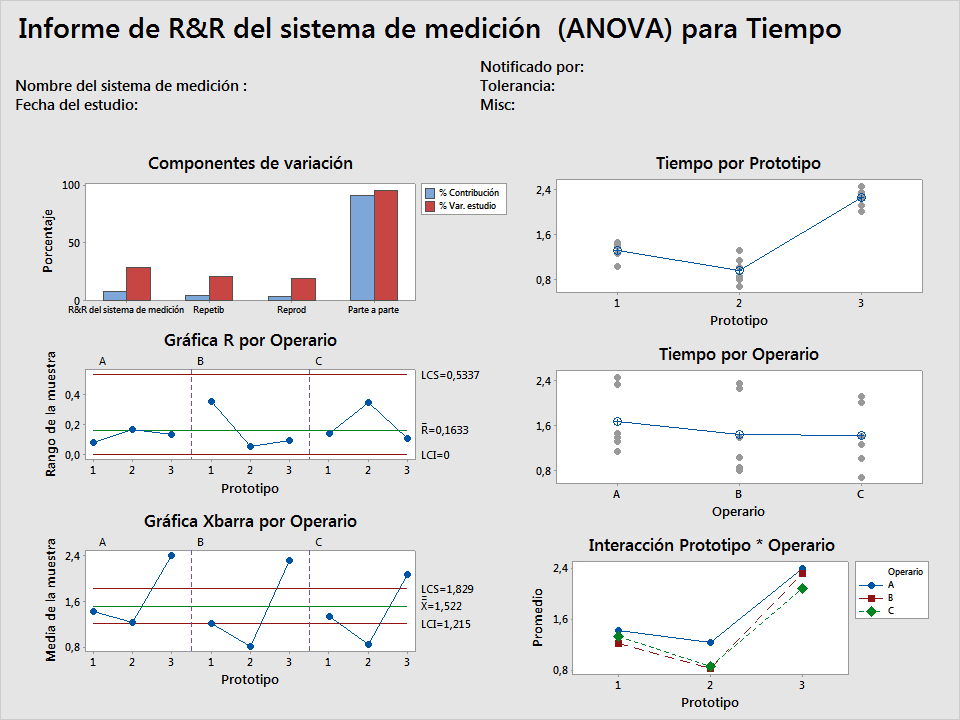
\includegraphics[width=0.7\linewidth]{imagenes/RR_del_sistema_de_medicion_para_Tiempo}
	\caption{R\&R del sistema de medición}
	\label{fig:R&RdelsistemademediciónparaTiempo}
\end{figure}

Ahora, procedemos a realizar el análisis de capacidad del proceso actual. Para ello, tomamos 20 medidas del tiempo de vuelo para un mismo prototipo. En nuestro caso, el prototipo 2. Los tiempos de vuelo recogidos se pueden ver la Tabla~\ref{tbl:tiempos_capacidad}.\\

\begin{center}
	\begin{longtable}{ccc}
		\caption{Tiempos de vuelo del prototipo 2 para calcular la capacidad del proceso}\\
		\label{tbl:tiempos_capacidad} \\
		\hline
		Tiempo \\
		\hline
		\endfirsthead
		\multicolumn{1}{c}%
		{\tablename\ \thetable\ -- \textit{Continúa de la página anterior}} \\
		\hline
		Tiempo \\
		\hline
		\endhead
		\hline \multicolumn{1}{r}{\textit{Continúa en la página siguiente}} \\
		\endfoot
		\hline
		\endlastfoot
		1.150  \\
		1.574  \\
		1.210  \\
		1.471  \\
		1.234  \\
		1.294  \\
		1.471  \\
		1.057  \\
		1.138  \\
		1.110  \\
		0.971  \\
		1.067  \\
		1.072  \\
		1.199  \\
		1.177  \\
		1.305  \\
		1.287  \\
		1.188  \\
		0.964  \\
		1.134  \\
	\end{longtable}
\end{center}

Antes de calcular la capacidad del proceso, comprobamos si los datos están distribuidos de acuerdo a una distribución normal. Para ello, aplicamos el test de Anderson-Darling en Minitab. Los resultados de este test se pueden ver en la Figura~\ref{fig:normalidad_capacidad}.\\

\begin{figure}[htbp!]
	\centering
	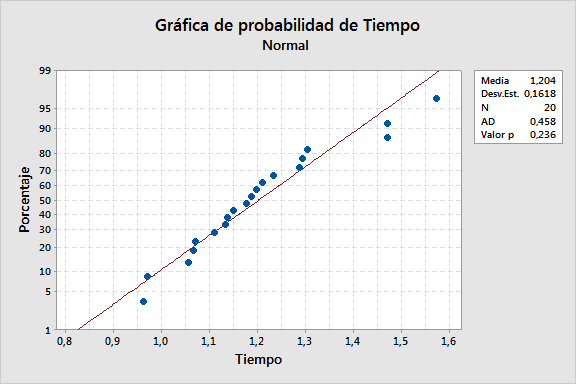
\includegraphics[width=0.7\linewidth]{imagenes/Grafica_de_normalidad_de_Tiempo_(analisis_de_capacidad)}
	\caption{Resultado del test de Anderson-Darling}
	\label{fig:normalidad_capacidad}
\end{figure}

El test arroja un p-valor de 0.236, mayor que 0.05. Por lo que no tenemos evidencia para rechazar la hipótesis de que los datos siguen una distribución normal.\\

Ya estamos en disposición de calcular la capacidad del proceso actual. El resultado del análisis de capacidad se puede ver en la Figura~\ref{fig:capacidad_actual}.\\ 

\begin{figure}[htbp!]
	\centering
	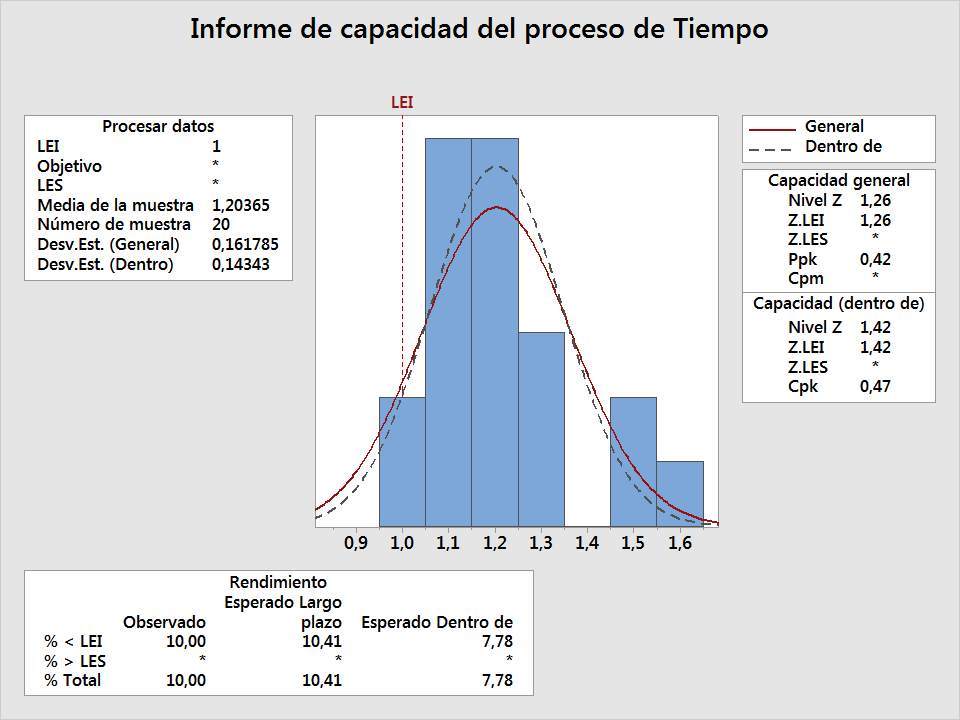
\includegraphics[width=0.7\linewidth]{imagenes/Informe_de_capacidad_del_proceso_de_Tiempo}
	\caption{Análisis de capacidad del proceso actual}
	\label{fig:capacidad_actual}
\end{figure}

Vemos que nuestro proceso tiene 1.26 sigmas, por lo que tenemos un gran margen de mejora en el proceso actual. Si siguiéramos con este proceso a largo plazo, nuestro proceso mejoraría hasta las 1.42 sigmas, insuficiente para los objetivos que marca el cliente.\\

Antes de analizar las causas que influyen en el tiempo de vuelo de nuestro helicóptero, debemos determinar las causas que pueden afectar al tiempo de vuelo. Para ello, aplicamos la regla de las 6 M's (mediciones, material, personal, medio ambiente, métodos y máquinas)\\

En el grupo de las mediciones identificamos como causas el largo de ala, el ancho del cuerpo y largo del cuerpo. En material identificamos la calidad y el peso. En personal, la experiencia, la motivación y la formación. En el medio ambiente, la velocidad del viento. En métodos la calidad del corte, del doblado y del pegado y la prueba de vuelo. Por último, en máquinas identificamos la edad y el mantenimiento. Todo esto se puede ver de forma gráfica en el diagrama de causas y efectos o diagrama de Ishikawa (Figura~\ref{fig:causa_efecto}).\\


\begin{figure}[htbp!]
	\centering
	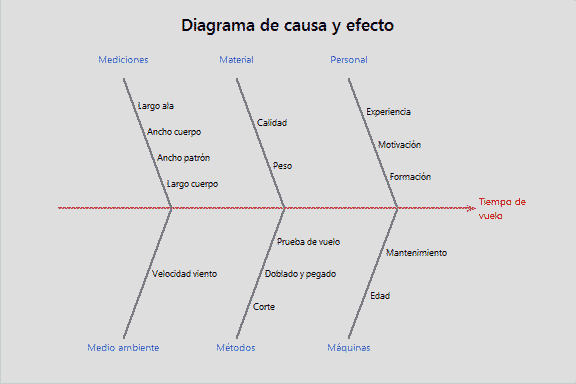
\includegraphics[width=0.7\linewidth]{imagenes/Diagrama_de_causa_y_efecto}
	\caption{Diagrama de causas y efectos para el tiempo de vuelo}
	\label{fig:causa_efecto}
\end{figure}


\section{Análisis gráfico}

Con las causas definidas que pueden causar las variaciones en el tiempo de vuelo de nuestros helicópteros, procedemos a analizar tanto desde un punto gráfico como numérico. Sólo nos centraremos en las condiciones de diseño (largo del ala, largo del cuerpo, ancho del cuerpo, si tiene clip o no, etc) y los operarios. Las causas como el mantenimiento de las herramientas o la edad las consideramos irrelevantes para el tiempo de vuelo.\\

Con los datos recogidos para el sistema de medición (Tabla~\ref{tbl:tiempos_operario}) y para la capacidad del proceso (Tabla~\ref{tbl:tiempos_capacidad}) analizamos de forma gráfica estos datos con la ayuda de Minitab.\\

En primer lugar, analizamos la normalidad de los datos del sistema de medición. Aplicamos el test de Anderson-Darling con Minitab. Los resultados de este test se pueden ver en la Figura~\ref{fig:normalidad_rr}.\\

\begin{figure}[htbp!]
	\centering
	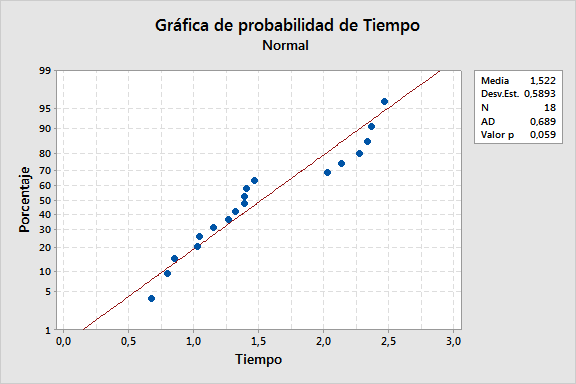
\includegraphics[width=0.7\linewidth]{imagenes/Grafica_de_normalidad_de_Tiempo_(datos_RR)}
	\caption{Resultados del test de normalidad para los datos del sistema de medida}
	\label{fig:normalidad_rr}
\end{figure}

Podemos observar que el p-valor es 0.059, mayor que 0.05, por lo que no hay evidencias para rechazar la hipótesis de que los datos sigan una distribución normal.\\

Ahora, podemos comprobar los efectos de cada factor (prototipo y operario) sobre el tiempo de vuelo. Para ello, aplicamos un diagrama de efectos principales. La Figura~\ref{fig:efectos_principales} muestra los resultados de este diagrama.\\

\begin{figure}[htbp!]
	\centering
	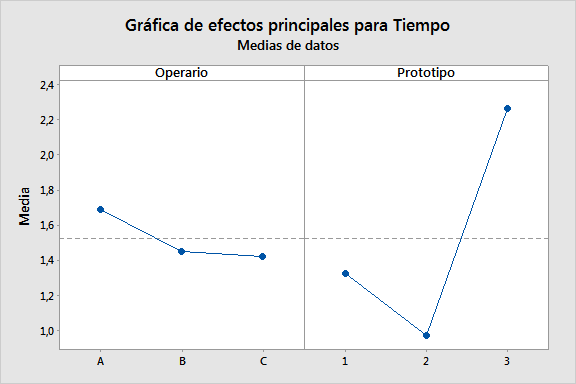
\includegraphics[width=0.7\linewidth]{imagenes/Grafica_de_efectos_principales_para_Tiempo}
	\caption{Diagrama de efectos principales para el tiempo de vuelo}
	\label{fig:efectos_principales}
\end{figure}

Se puede observar que entre los tiempos medios de vuelo para cada uno de los operarios (A, B, C) no hay una gran diferencia, lo que hace indicar que el operario que realice el helicóptero apenas influye en el tiempo de vuelo. Sin embargo, en los tiempos medios según el prototipo, existen grandes diferencias de tiempo. El que más sobresale es el prototipo número 3, que parece indicar que la combinación de las variables de diseño (longitud del ala, longitud del cuerpo, anchura del cuerpo, con clip o sin clip, etc) parece influir bastante en el tiempo de vuelo.\\

A continuación, analizamos el tiempo de vuelo según el prototipo realizando gráficas de efectos principales como en el caso anterior (Figura~\ref{fig:efectos_principales_prototipos}).

\begin{figure}[htbp!]
	\centering
	\subfigure[Prototipo 1]{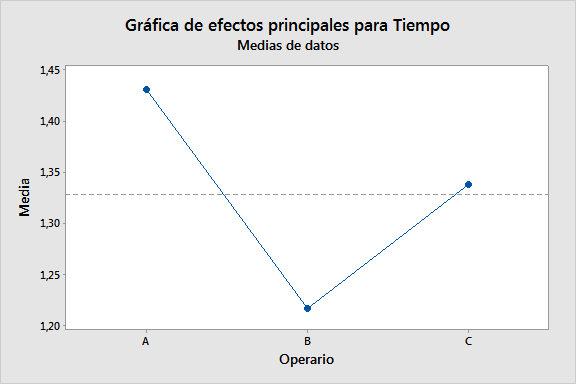
\includegraphics[width=0.45\linewidth]{imagenes/Grafica_de_efectos_principales_para_Tiempo_(Prototipo_1)}}
	\subfigure[Prototipo 2]{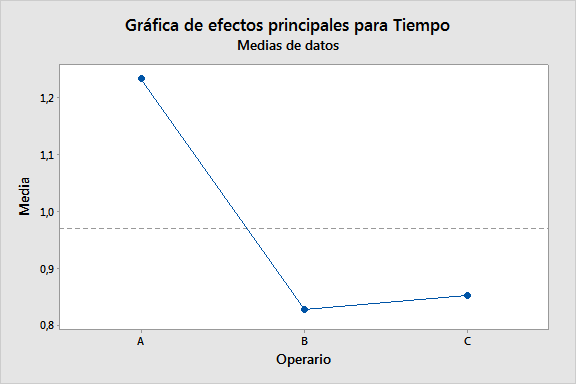
\includegraphics[width=0.45\linewidth]{imagenes/Grafica_de_efectos_principales_para_Tiempo_(Prototipo_2)}}
	\subfigure[Prototipo 3]{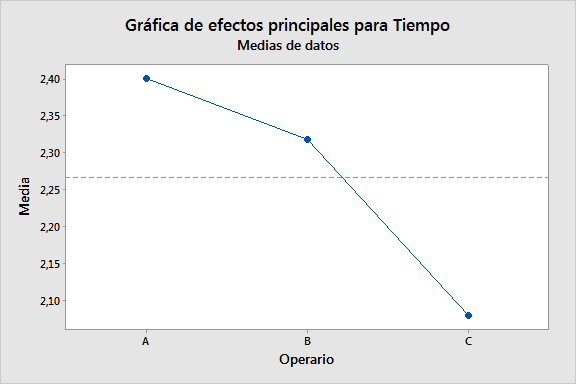
\includegraphics[width=0.45\linewidth]{imagenes/Grafica_de_efectos_principales_para_Tiempo_(Prototipo_3)}}
	\caption{Diagrama de efectos principales para el tiempo según el tipo de prototipo} \label{fig:efectos_principales_prototipos}
\end{figure}

Observamos que los tiempos según el tipo de prototipo, sí parece estar influido por el operario que realizó el helicóptero. En el caso del prototipo 1, el mayor tiempo medio se consiguió con el operario A, aunque todos cumplen con el objetivo mínimo del tiempo de vuelo fijado por el cliente. En el prototipo 2, de nuevo, el mayor tiempo de vuelo se consigue con el operario A, pero con los operarios B y C no se consigue el objetivo mínimo de 1 segundo de vuelo. Por último, con el prototipo 3, se cumple de sobra con el objetivo mínimo de tiempo de vuelo, y con el operario A se realizan los mejores tiempos de vuelo. Parece que el operario A es el que mejor realiza los helicóptero, ya que con él se consiguen los mejores tiempos de vuelo (independientemente del prototipo elegido).\\

A continuación, analizamos la capacidad de cada uno de los procesos si sólo fabricáramos un solo tipo de prototipo (Figura~\ref{fig:capacidad_prototipos}).\\

\begin{figure}[htbp!]
	\centering
	\subfigure[Prototipo 1]{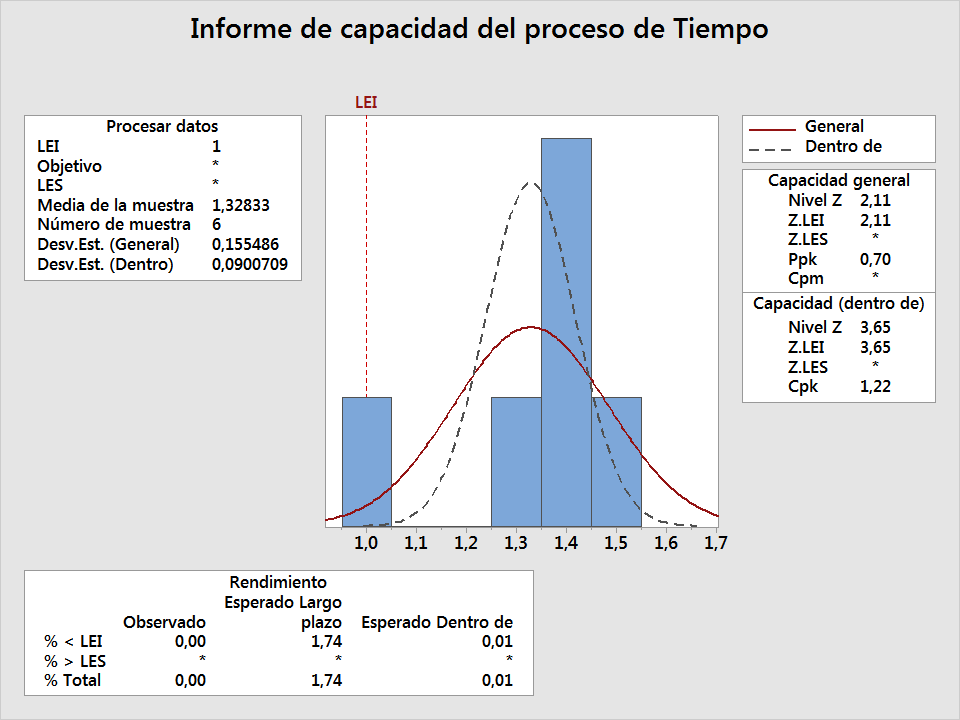
\includegraphics[width=0.45\linewidth]{imagenes/Informe_de_capacidad_del_proceso_de_Tiempo_(Prototipo_1)}}
	\subfigure[Prototipo 2]{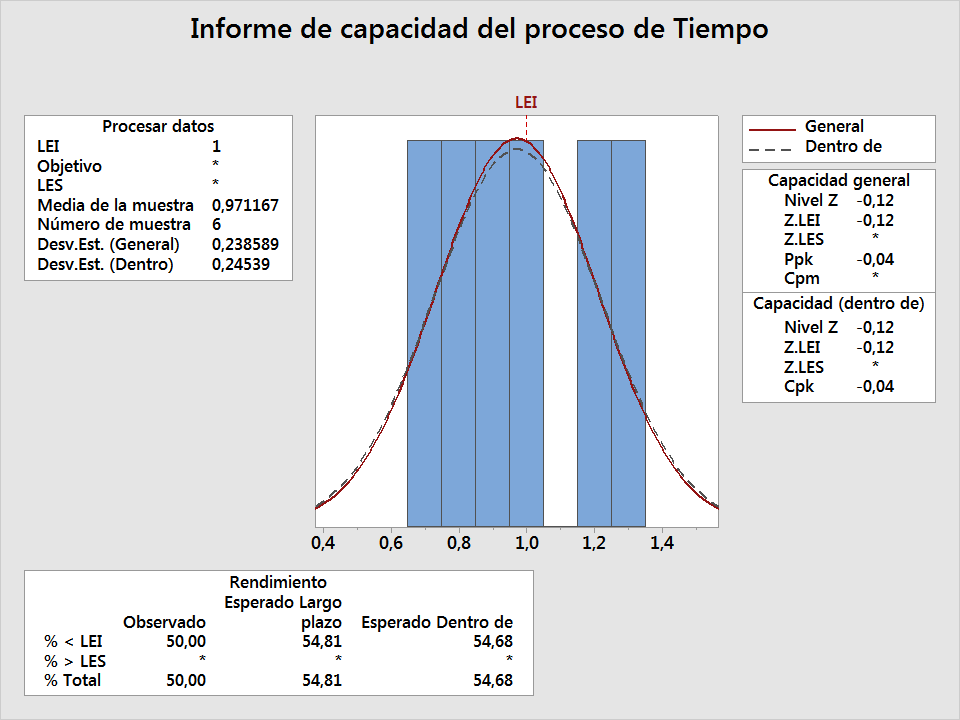
\includegraphics[width=0.45\linewidth]{imagenes/Informe_de_capacidad_del_proceso_de_Tiempo_(Prototipo_2)}}
	\subfigure[Prototipo 3]{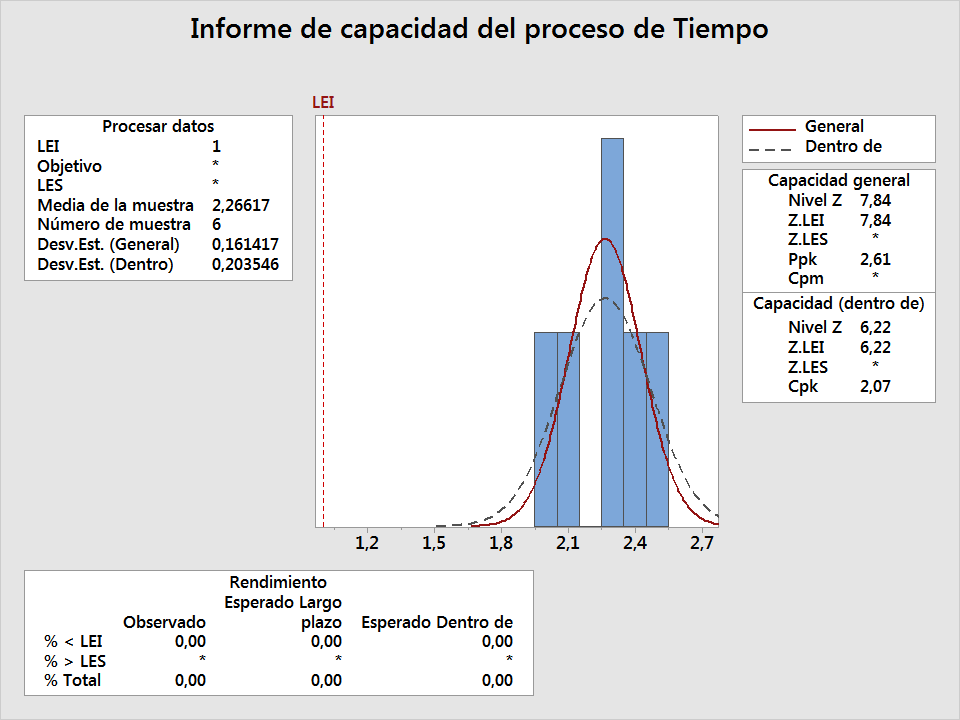
\includegraphics[width=0.45\linewidth]{imagenes/Informe_de_capacidad_del_proceso_de_Tiempo_(Prototipo_3)}}
	\caption{Capacidad del proceso según el tipo de prototipo} \label{fig:capacidad_prototipos}
\end{figure}

Si sólo fabricáramos prototipos como el número 1, nuestros proceso mejoraría hasta las 2.11 sigmas a corto plazo. En el caso del prototipo 2, tenemos un proceso de -0.12 sigmas. Debido al pequeño tamaño muestral $n=6$, consideraremos esta capacidad como no válida, y usaremos el nivel obtenido en la Figura~\ref{fig:capacidad_actual}. Recordar que la capacidad del proceso se calculó usando sólo prototipos del segundo tipo. El tercer prototipo, tiene una capacidad de 7.84 sigmas, que cumple con los objetivos de calidad. Es de esperar que para obtener la calidad pedida por el cliente, necesitemos fabricar los helicópteros más parecidos a las especificaciones del tercer prototipo que a los de los otros dos. \\

A continuación, realizamos un histograma para de cada uno de los tipos de prototipo (Figura~\ref{fig:histograma}).

\begin{figure}[htbp!]
	\centering
	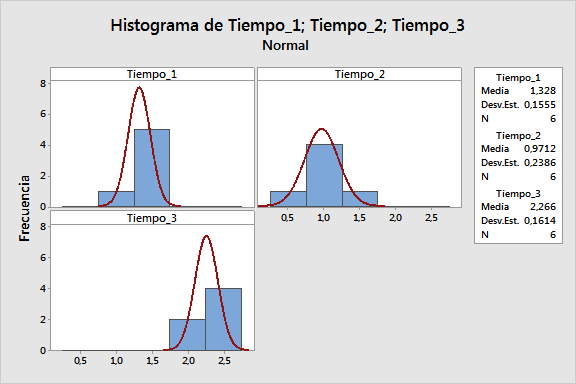
\includegraphics[width=0.7\linewidth]{imagenes/Histograma_de_Tiempo_1_Tiempo_2_Tiempo_3_(por_prototipo)}
	\caption{Histograma según el tipo de prototipo}
	\label{fig:histograma}
\end{figure}

Se puede observar como el prototipo que obtiene mayores tiempos es el número 3, superando los dos segundos de vuelo, el tiempo del prototipo 1 se sitúa en torno a 1.4-1.5 segundos de vuelo, mientras que el prototipo 2 tiene una media que no llega al segundo, y por tanto, no cumple el tiempo mínimo fijado por el cliente. Aunque, hay que tener en cuenta que estamos con una muestra muy pequeña $n=6$.\\

A continuación realizamos una gráfica de serie temporal, según el tipo de prototipo (Figura~\ref{fig:temporal}).\\

\begin{figure}[htbp!]
	\centering
	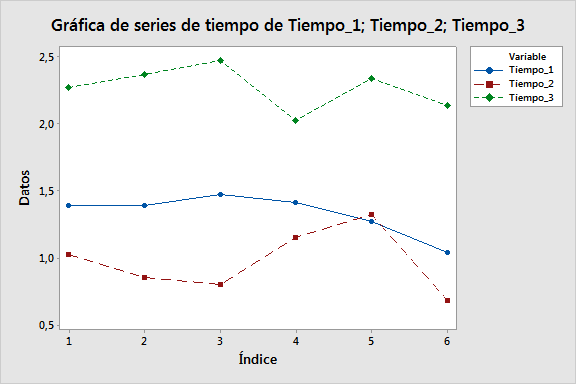
\includegraphics[width=0.7\linewidth]{imagenes/Grafica_de_series_de_tiempo_de_Tiempo_1;_Tiempo_2;_Tiempo_3}
	\caption{Diagrama de serie temporal según el prototipo}
	\label{fig:temporal}
\end{figure}

Vemos que el prototipo 3 es el que mayor tiempo de vuelo tiene, superando con mucha diferencia a los otros dos prototipos. El prototipo 1 mantiene el tiempo de vuelo mucho más uniforme, siempre por encima de los límites de calidad especificados. Por el contrario, el prototipo 2 no llega al límite de calidad en la mayoría de las veces.\\

Si representamos ahora el diagrama de puntos (Figura~\ref{fig:diagrama_puntos}), vemos que existen dos tiempos de vuelos: los que son superiores a los 2 segundos y los que son inferiores a 1.5 segundos. Los primeros corresponden a los del prototipo 3, mientras que los segundos vienen de los prototipos 1 y 2.\\

También observamos 3 datos que están por debajo del tiempo especificado. Éstos se corresponden con los obtenidos del prototipo 2.\\ 

\begin{figure}[htbp!]
	\centering
	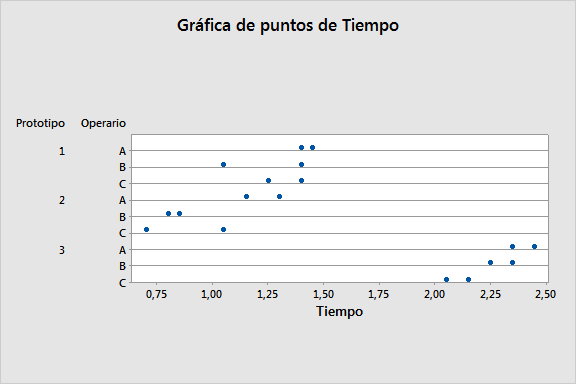
\includegraphics[width=0.7\linewidth]{imagenes/Grafica_de_puntos_de_Tiempo}
	\caption{Diagrama de puntos para el tiempo de vuelo}
	\label{fig:diagrama_puntos}
\end{figure}

Si, por último, representamos un diagrama de cajas (Figura~\ref{fig:diagrama_cajas}), vemos que el prototipo 3 es el que mayor tiempo de vuelo tiene, aunque con el operario C es con el que menor tiempo se consigue. Los tiempos del prototipo 1 varían poco, salvo en el caso del operario B que sus tiempos tienen mayor amplitud, aunque dentro del límite marcado. Los tiempos del prototipo 2, con el operario A, están dentro de los límites especificados. Con el operario B, están todos fuera y los del operario C hay algunos que están dentro y otros fuera. 

\begin{figure}[htbp!]
	\centering
	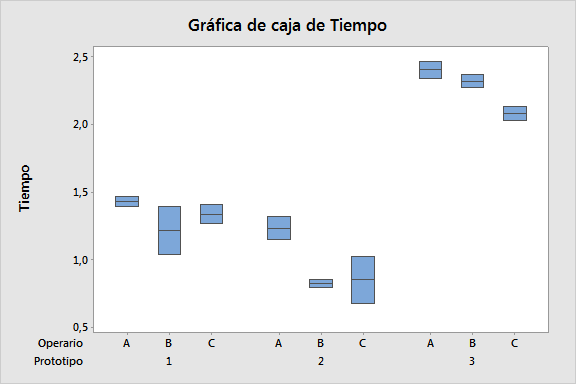
\includegraphics[width=0.7\linewidth]{imagenes/Grafica_de_caja_de_Tiempo}
	\caption{Diagrama de cajas para el tiempo de vuelo}
	\label{fig:diagrama_cajas}
\end{figure}

En definitiva, hemos visto que el prototipo con mayor tiempo de vuelo es el 3, seguido del 1. El único que no cumplía los objetivos de calidad es el prototipo 2.

\subsection{Análisis numérico}

A continuación realizaremos una serie de contrastes de hipótesis para conocer si existen diferencias significativas entre los tiempos medios según distintas variables.\\

Comenzaremos con la variable Clip. Tenemos que contrastar si las medidas de los tiempos de vuelo entre los helicópteros con clip o sin él son significativas. Es decir:

\begin{eqnarray*}
\begin{cases}
	H_0: \mu_{\text{Clip = sí}} = \mu_{\text{Clip = no}} \\
	H_1: \mu_{\text{Clip = sí}} \neq \mu_{\text{Clip = no}}
\end{cases}
\end{eqnarray*}

Resolviendo este contraste de hipótesis con Minitab, tenemos los resultados que se muestran a continuación:

\begin{verbatim}
T de dos muestras para Clip=si vs. Clip=no

                                 Error
                              estándar
                                 de la
         N  Media  Desv.Est.     media
Clip=si  6  1,061      0,283      0,12
Clip=no  6  2,266      0,161     0,066


Diferencia = μ (Clip=si) - μ (Clip=no)
Estimación de la diferencia:  -1,205
IC de 95% para la diferencia:  (-1,520; -0,891)
Prueba T de diferencia = 0 (vs. ≠): Valor T = -9,07                               Valor p = 0,000  GL = 7
\end{verbatim}

Es decir, p-valor = 0.000 < 0.05, por lo que rechazamos $H_0$ y existen diferencias significativas entre los tiempos de vuelo de los helicópteros cuando llevan o no llevan un clip. Es más, cuando no lo llevan el tiempo de vuelo es mayor: de media será 1.205 segundos y en el 95\% de los casos estará entre 0.891 y 1.5220 segundos más que no llevar clip.\\

Ahora analizaremos si la longitud del cuerpo influye en el tiempo de vuelo. Tenemos dos medidas de la longitud del cuerpo: 6.5 y 8.0 cm. El constaste de hipótesis en el siguiente:

\begin{eqnarray*}
	\begin{cases}
		H_0: \mu_{\text{Largo\_cuerpo = 6.5}} = \mu_{\text{Largo\_cuerpo = 8.0}} \\
		H_1: \mu_{\text{Largo\_cuerpo = 6.5}} \neq \mu_{\text{Largo\_cuerpo = 8.0}}
	\end{cases}
\end{eqnarray*}

Los resultados que devuelve Minitab son los siguientes:

\begin{verbatim}
T de dos muestras para Largo_cuerpo=8 vs. Largo_cuerpo=6,5

                                           Error
                                        estándar
                                           de la
                   N  Media  Desv.Est.     media
Largo_cuerpo=8    12  1,195      0,259     0,075
Largo_cuerpo=6,5   6  2,266      0,161     0,066


Diferencia = μ (Largo_cuerpo=8) - μ (Largo_cuerpo=6,5)
Estimación de la diferencia:  -1,0716
IC de 95% para la diferencia:  (-1,2851; -0,8580)
Prueba T de diferencia = 0 (vs. ≠): Valor T = -10,76  
                                    Valor p = 0,000  GL = 14
\end{verbatim}

Vemos que el p-valor=0.000 < 0.05, por lo que tenemos que rechazar $H_0$ y aceptar que existen diferencias significativas en los tiempos de vuelo, según la longitud del cuerpo del helicóptero. De hecho, el mayor tiempo de vuelo se da cuando la longitud del cuerpo es de 6.5 cm. La estimación de la diferencia es de 1.0716 con respecto a la longitud del cuerpo de 8.5 cm. Y en el 95\% de los casos estará entre 0.8580 y 1.2851 segundos de diferencia en el tiempo de vuelo. \\

Por último, realizaremos un contraste de hipótesis para ver si existen diferencias entre los helicópteros (con clip) con longitud de ala igual a 8.0 y los que tienen longitud de ala de 6.5 cm. El contraste de hipótesis es el siguiente:

\begin{eqnarray*}
	\begin{cases}
		H_0: \mu_{\text{Largo\_ala = 6.5}} = \mu_{\text{Largo\_ala = 8.0}} \\
		H_1: \mu_{\text{Largo\_ala = 6.5}} \neq \mu_{\text{Largo\_ala = 8.0}}
	\end{cases}
\end{eqnarray*}

Los resultados del test son los siguientes:

\begin{verbatim}
T de dos muestras para Largo_ala=8 vs. Largo_ala=6,5

                                       Error
                                    estándar
                                       de la
               N  Media  Desv.Est.     media
Largo_ala=8    6  1,328      0,155     0,063
Largo_ala=6,5  6  1,061      0,283      0,12


Diferencia = μ (Largo_ala=8) - μ (Largo_ala=6,5)
Estimación de la diferencia:  0,268
IC de 95% para la diferencia:  (-0,044; 0,579)
Prueba T de diferencia = 0 (vs. ≠): Valor T = 2,03  
                                    Valor p = 0,082  GL = 7
\end{verbatim}

Vemos que el p-valor = 0.082 > 0.05, por lo que no hay evidencias para rechazar $H_0$, por lo que tenemos que apenas hay diferencia entre los tiempos de vuelo cuando el helicóptero lleva clip y la longitud de las alas está entre 6.5 y 8.0 cm. La diferencia media está en 0.268 segundos para la longitud de ala igual a 8 (es decir, esta longitud de ala da una pequeña mejora en el tiempo de vuelo, apenas significativo con respecto a la longitud de 6.5 cm).\\

Acabamos de ver que entre los helicópteros con clip, un largo de ala entre 6.5 y 8 cm. apenas aporta nada de tiempo de vuelo al helicóptero, pero no sabemos nada de cómo influye en los helicópteros sin clip. Para ello, tomamos una serie de tiempos con helicópteros del prototipo 3 (el único que no lleva clip), con distintas longitudes de ala (desde 6.5 hasta 9.5). Los datos se pueden ver en la Tabla~\ref{tbl:regresion}.\\


\begin{table}[htbp!]
	\centering
	\caption{Tiempos de distintos longitudes de ala para el prototipo 3}
	\label{tbl:regresion}
	\begin{tabular}{@{}cc@{}}
		\toprule
		Largo ala & Tiempo \\ \midrule
		9.5       & 2.039  \\
		9.5       & 2.101  \\
		9.5       & 2.320  \\
		8.5       & 2.135  \\
		8.5       & 1.885  \\
		8.5       & 1.949  \\
		7.5       & 1.766  \\
		7.5       & 1.812  \\
		7.5       & 1.542  \\
		6.5       & 1.380  \\
		6.5       & 1.340  \\
		6.5       & 1.277  \\ \bottomrule
	\end{tabular}
\end{table}

Vamos a ver si existe una relación lineal entre estas dos variables, con la ayuda del análisis de regresión. Los resultados de este análisis se pueden ver a continuación:

\begin{verbatim}
La ecuación de regresión es
Tiempo = - 0,4013 + 0,2746 Largo ala


S = 0,125637   R-cuad. = 87,8%   R-cuad.(ajustado) = 86,5%


Análisis de Varianza

Fuente     GL       SC       MC      F      P
Regresión   1  1,13108  1,13108  71,66  0,000
Error      10  0,15785  0,01578
Total      11  1,28892
\end{verbatim}

Vemos que existe una fuerte relación lineal entre estas dos variables, teniendo un coeficiente de determinación ajustado $R^2$ de 0.865, lo que indica un ajuste bastante bueno.\\

La recta de regresión es la siguiente:

\begin{equation*}
\text{Tiempo} = -0.4013 + 0.2746 \cdot \text{Largo ala}
\end{equation*}

La recta de regresión junto con el diagrama de dispersión se muestra en la Figura~\ref{fig:regresion}.\\

\begin{figure}[htbp!]
	\centering
	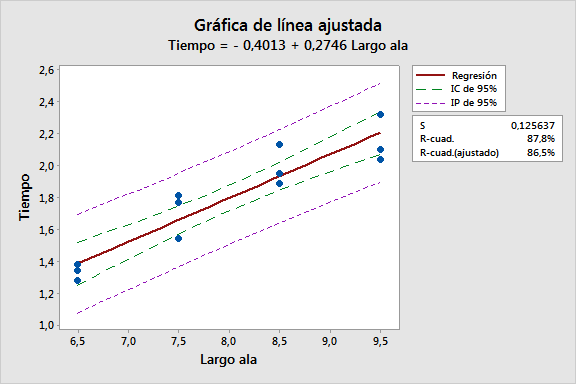
\includegraphics[width=0.7\linewidth]{imagenes/Linea_ajustada__Tiempo_vs}
	\caption{Recta de regresión para el tiempo y la longitud del ala}
	\label{fig:regresion}
\end{figure}

Observamos que la gran mayoría de los datos se encuentran dentro del intervalo de probabilidad del 95\%.\\

Sólo nos queda verificar que todas las hipótesis del modelo de regresión se cumplen. Para ello, hacemos un análisis de los residuos del modelo (Figura~\ref)\\

\begin{figure}[htbp!]
	\centering
	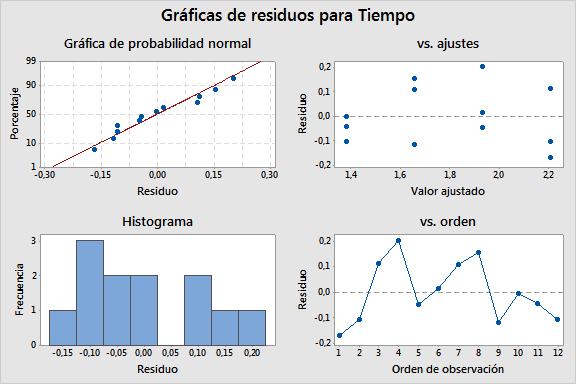
\includegraphics[width=0.7\linewidth]{imagenes/Graficas_de_residuos_para_Tiempo_(regresion)}
	\caption{Análisis de residuos para el modelo de regresión}
	\label{fig:residuos_regresion}
\end{figure}

Nada parece indicar que se viole alguna de las hipótesis de partida: los residuos se distribuyen según una distribución normal, la varianza de los residuos no depende del predictor y la independencia de los residuos.\\

A continuación, usamos ANOVA para identificar las variables significativas que afectan al tiempo de vuelo.\\

Comenzamos por la variable Clip. Lo primero de todo es comprobar si se cumplen las hipótesis del modelo: independencia, homocedasticidad y normalidad. \\

Comprobamos la normalidad. El resumen se muestra en la Figura~\ref{fig:normalidad_clip}.\\ 

\begin{figure}[htbp!]
	\centering
	\subfigure[Clip=sí]{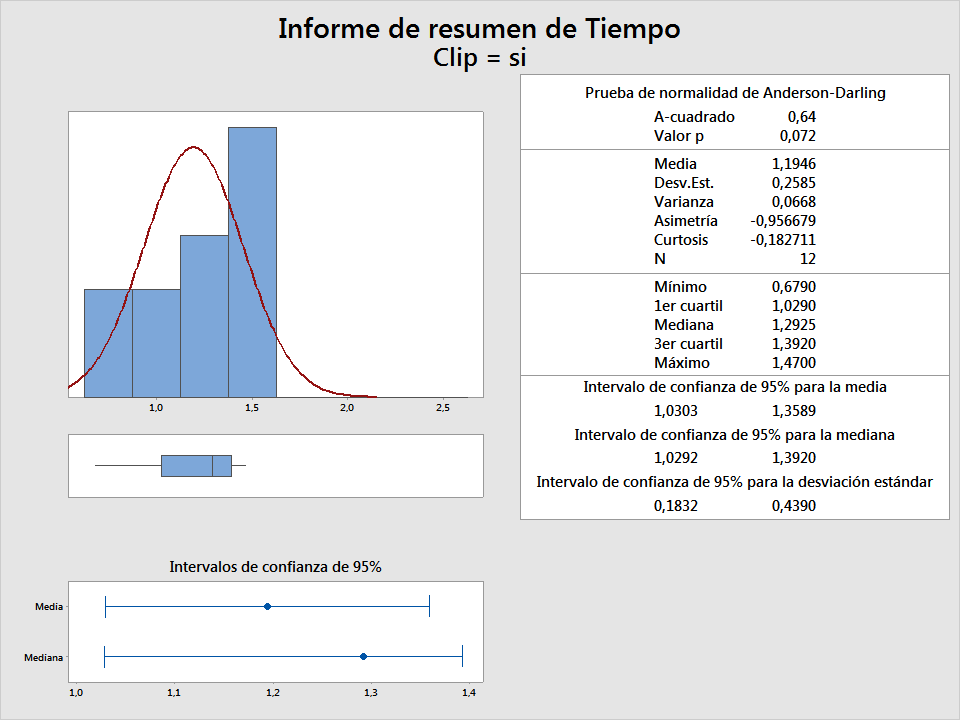
\includegraphics[width=0.45\linewidth]{imagenes/Informe_de_resumen_de_Tiempo(Clip=si)}}
	\subfigure[Clip=no]{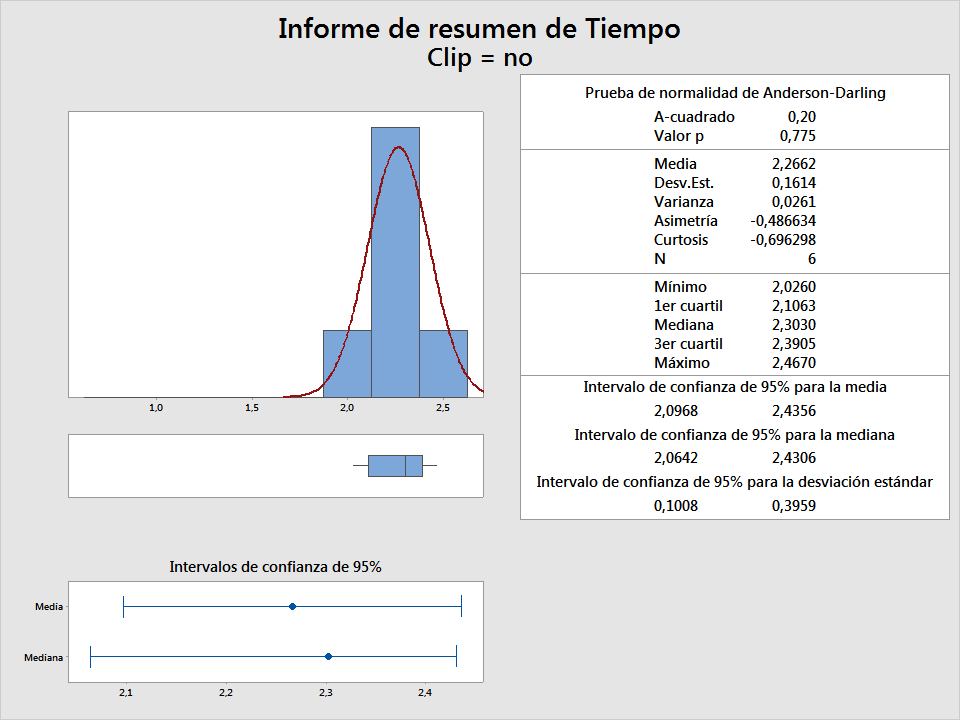
\includegraphics[width=0.45\linewidth]{imagenes/Informe_de_resumen_de_Tiempo(Clip=no)}}
	\caption{Resumen de la variable Clip} \label{fig:normalidad_clip}
\end{figure}

El p-valor del test de Anderson-Darling indica que cada subgrupo es normal, por lo que se cumple esta hipótesis.\\

Ahora comprobamos la independencia. La correlación entre variables se muestra a continuación:

\begin{verbatim}
Correlación de Pearson de Clip=si y Clip=no = -0,672
Valor p = 0,144
\end{verbatim}

Puesto que el p-valor es mayor que 0.05, podemos asumir independencia.\\

Sólo nos queda comprobar la homocedasticidad (o igualdad de varianzas). El resultado del test es el siguiente:

\begin{verbatim}
Método

Hipótesis nula          Todas las varianzas son iguales
Hipótesis alterna       Por lo menos una varianza es diferente
Nivel de significancia  α = 0,05


Intervalos de confianza de Bonferroni de 95% para desviaciones estándar

Muestra  N  Desv.Est.           IC
Clip=si  6   0,282756  (0,146390; 0,871845)
Clip=no  6   0,161417  (0,063302; 0,657064)

Nivel de confianza individual = 97,5%


Pruebas

                         Estadística
Método                     de prueba  Valor p
Comparaciones múltiples         1,74    0,187
Levene                          2,23    0,166

\end{verbatim}

Puesto que el p-valor es mayor que 0.05, no hay evidencia estadística para rechazar la igualdad de varianzas.\\

Tenemos, por tanto, un modelo válido. Procedemos a analizarlo.\\

\begin{verbatim}
Método

Hipótesis nula          Todas las medias son iguales
Hipótesis alterna       Por lo menos una media es diferente
Nivel de significancia  α = 0,05

Se presupuso igualdad de varianzas para el análisis.


Información del factor

Factor  Niveles  Valores
Factor        2  Clip=si; Clip=no


Análisis de Varianza

Fuente  GL  SC Ajust.  MC Ajust.  Valor F  Valor p
Factor   1     4,3585    4,35849    82,23    0,000
Error   10     0,5300    0,05300
Total   11     4,8885


Resumen del modelo

                      R-cuad.  R-cuad.
       S  R-cuad.  (ajustado)   (pred)
0,230224   89,16%      88,07%   84,39%


Medias

Factor   N   Media  Desv.Est.      IC de 95%
Clip=si  6   1,061      0,283  ( 0,851;  1,270)
Clip=no  6  2,2662     0,1614  (2,0567; 2,4756)

Desv.Est. agrupada = 0,230224

\end{verbatim}

Existen diferencias significativas entre el tiempo medio de vuelo de los helicópteros con clip o sin clip. Este resultado sólo confirma lo que ya sabíamos: que el clip influye en el tiempo de vuelo de los helicópteros.\\

Ahora analizaremos la variable largo del ala. Representamos su resumen de residuos para ver que se cumplen todas las hipótesis del modelo (Figura~\ref{fig:residuos_largo_ala}).\\

\begin{figure}[htbp!]
	\centering
	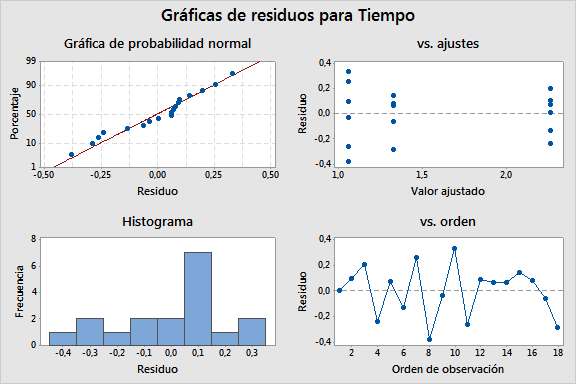
\includegraphics[width=0.7\linewidth]{imagenes/Graficas_de_residuos_para_Tiempo_(ANOVA_largo_ala)}
	\caption{Análisis de residuos para la longitud del ala}
	\label{fig:residuos_largo_ala}
\end{figure}

Nada parece indicar una violación de las hipótesis de partida.\\

Analizamos el modelo, con los resultados siguientes:

\begin{verbatim}
Método

Hipótesis nula          Todas las medias son iguales
Hipótesis alterna       Por lo menos una media es diferente
Nivel de significancia  α = 0,05

Se presupuso igualdad de varianzas para el análisis.


Información del factor

Factor     Niveles  Valores
Largo ala        3  6,5; 8,0; 9,5


Análisis de Varianza

Fuente     GL  SC Ajust.  MC Ajust.  Valor F  Valor p
Largo ala   2     4,8078    2,40392    55,40    0,000
Error      15     0,6509    0,04339
Total      17     5,4587


Resumen del modelo

                      R-cuad.  R-cuad.
       S  R-cuad.  (ajustado)   (pred)
0,208312   88,08%      86,49%   82,83%


Medias

Largo
ala    N   Media  Desv.Est.      IC de 95%
6,5    6   1,061      0,283  ( 0,880;  1,242)
8,0    6  1,3283     0,1555  (1,1471; 1,5096)
9,5    6  2,2662     0,1614  (2,0849; 2,4474)

Desv.Est. agrupada = 0,208312
\end{verbatim}

Puesto que el p-valor es menor que 0.05, podemos afirmar que existe al menos un tiempo medio que no se corresponde con los demás.\\

Representamos el tiempo de vuelo según estos factores (Figura~\ref{fig:resultado_largo_alas}).\\

\begin{figure}[htbp!]
	\centering
	\subfigure[Gráfica de cajas]{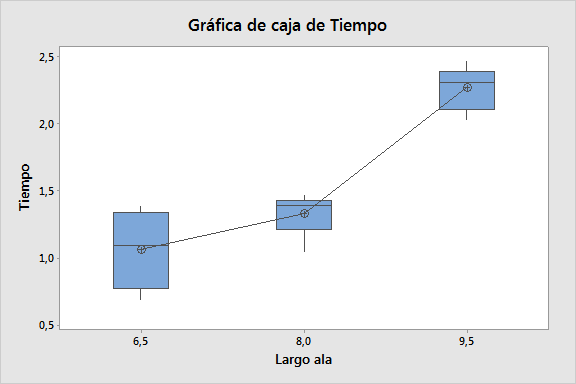
\includegraphics[width=0.45\linewidth]{imagenes/Grafica_de_caja_de_Tiempo_(ANOVA_largo_ala)}}
	\subfigure[Gráfica de intervalos]{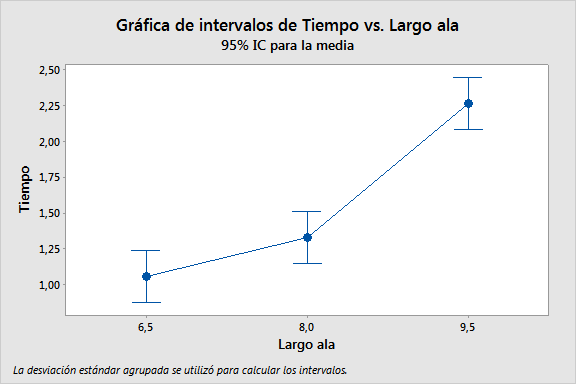
\includegraphics[width=0.45\linewidth]{imagenes/Grafica_de_intervalos_de_Tiempo_vs_(ANOVA_largo_ala)}}
	\caption{Resultado de la variable longitud de las alas} \label{fig:resultado_largo_alas}
\end{figure}

Vemos que el que proporciona más tiempo de vuelo es la longitud de 9.5 cm. Comparemos si existen diferencias significativas entre las longitudes de 6.5 y 8 cm. Esto lo habíamos calculado anteriormente, dando como resultado que no había diferencias entre las medias de los tiempos de vuelo con estas longitudes de ala.\\

Procedemos a analizar la variable longitud del cuerpo. Hacemos un análisis de los residuos del modelo que se pueden ver en la Figura~\ref{fig:residuos_largo_cuerpo}. 

\begin{figure}[htbp!]
	\centering
	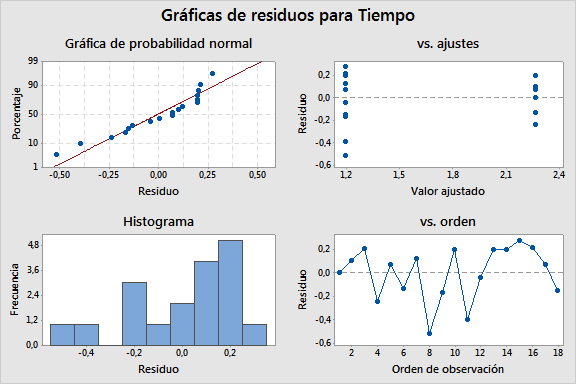
\includegraphics[width=0.7\linewidth]{imagenes/Graficas_de_residuos_para_Tiempo_ANOVA_(largo_cuerpo)}
	\caption{Análisis de residuos para la longitud del cuerpo}
	\label{fig:residuos_largo_cuerpo}
\end{figure}

Parece ser que no se incumple ninguna hipótesis de partida. Por tanto, estamos en disposición de analizar la variable. Los resultados se muestran a continuación:

\begin{verbatim}
Método

Hipótesis nula          Todas las medias son iguales
Hipótesis alterna       Por lo menos una media es diferente
Nivel de significancia  α = 0,05

Se presupuso igualdad de varianzas para el análisis.


Información del factor

Factor        Niveles  Valores
Largo cuerpo        2  6,5; 8,0


Análisis de Varianza

Fuente        GL  SC Ajust.  MC Ajust.  Valor F  Valor p
Largo cuerpo   1     4,5932    4,59316    84,90    0,000
Error         16     0,8656    0,05410
Total         17     5,4587


Resumen del modelo

                      R-cuad.  R-cuad.
       S  R-cuad.  (ajustado)   (pred)
0,232591   84,14%      83,15%   80,53%


Medias

Largo
cuerpo   N   Media  Desv.Est.      IC de 95%
6,5      6  2,2662     0,1614  (2,0649; 2,4675)
8,0     12  1,1946     0,2585  (1,0522; 1,3369)

Desv.Est. agrupada = 0,232591
\end{verbatim} 

Vemos que el p-valor es 0.000, rechazamos la hipótesis nula de que las medias son igual, y podemos afirmar que existen diferencias entre los tiempos de vuelo dependiendo de la longitud del cuerpo.\\

Para ver cómo influyen en el tiempo de vuelo, representamos el diagrama de intervalos y de caja (Figura~\ref{fig:resultado_largo_cuerpo}).\\

\begin{figure}[htbp!]
	\centering
	\subfigure[Gráfica de cajas]{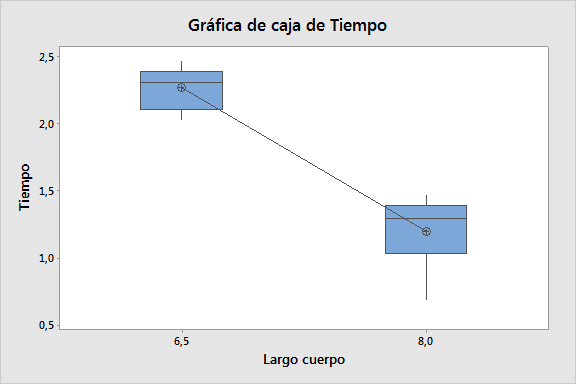
\includegraphics[width=0.45\linewidth]{imagenes/Grafica_de_caja_de_Tiempo_(ANOVA_largo_cuerpo)}}
	\subfigure[Gráfica de intervalos]{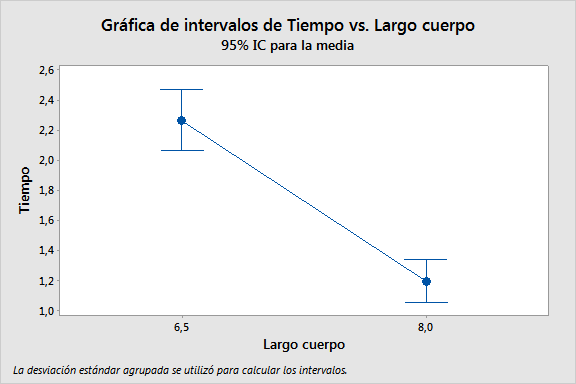
\includegraphics[width=0.45\linewidth]{imagenes/Grafica_de_intervalos_de_Tiempo_vs_(ANOVA_largo_cuerpo)}}
	\caption{Resultado de la variable longitud de las alas} \label{fig:resultado_largo_cuerpo}
\end{figure}

Vemos que la longitud que cuya longitud de cuerpo tiene mayor tiempo de vuelo es la de 6.5 cm, con un intervalo de confianza (al 95\%) de que el tiempo de vuelo está entre 2.0649 y 2.4675 segundos. Si nos fijamos en el intervalo de confianza para la longitud de 8 cm, vemos que el intervalo de confianza se sitúa entre 1.0522 y 1.3369, que cumple las especificaciones de calidad.\\

Por tanto, hay al menos tres variables que influyen en el tiempo de vuelo: llevar o no clip, el largo del ala y el largo del cuerpo. A continuación realizaremos unos experimentos para conocer la influencia de otras variables como llevar o no celo en el cuerpo o en ala o  el ancho del cuerpo.

\section{Mejora}

A continuación realizaremos una serie de experimentos para conocer las variables más significativas y las interacciones entre ellas que más influyen en el tiempo de vuelo de los helicópteros. Para ello, realizaremos dos experimentos: uno fraccional con fracción 1/2 y uno completo. Ambos experimentos tienen 6 factores con puntos centrales (entre paréntesis se indican los niveles): clip (sí, no), celo ala (sí, no), celo cuerpo (sí, no), largo ala (6.5, 9.5), largo cuerpo (6.5, 9.5)  y ancho cuerpo (4, 6).\\

Comenzaremos por el experimentos fraccional. Se trata, como hemos comentado anteriormente, de un diseño fraccional con fracción 1/2 con 6 factores. Los datos de este experimento se pueden ver el Anexo~\ref{chp:experimentos}. Analizamos el diseño factorial con la ayuda de Minitab. Los resultados de la salida (simplificada por su gran longitud) son los siguientes:

\begin{verbatim}
... (simplificado por brevedad)

Resumen del modelo

R-cuad.  R-cuad.
S  R-cuad.  (ajustado)   (pred)
*  100,00%           *        *

Término                      Valor T  Valor p   VIF
Constante                          *        *
Clip                               *        *  5,00
Celo_ala                           *        *  5,00
Celo_cuerpo                        *        *  5,00
Largo_ala                          *        *  1,00
Largo_cuerpo                       *        *  1,00
Ancho_cuerpo                       *        *  1,00
Clip*Celo_ala                      *        *  5,00
Clip*Celo_cuerpo                   *        *  5,00
Clip*Largo_ala                     *        *  1,00
Clip*Largo_cuerpo                  *        *  1,00
Clip*Ancho_cuerpo                  *        *  1,00
Celo_ala*Celo_cuerpo               *        *  5,00
Celo_ala*Largo_ala                 *        *  1,00
Celo_ala*Largo_cuerpo              *        *  1,00
Celo_ala*Ancho_cuerpo              *        *  1,00
Celo_cuerpo*Largo_ala              *        *  1,00
Celo_cuerpo*Largo_cuerpo           *        *  1,00
Celo_cuerpo*Ancho_cuerpo           *        *  1,00
Largo_ala*Largo_cuerpo             *        *  1,00
Largo_ala*Ancho_cuerpo             *        *  1,00
Largo_cuerpo*Ancho_cuerpo          *        *  1,00
Clip*Celo_ala*Celo_cuerpo          *        *  5,00
Clip*Celo_ala*Largo_ala            *        *  1,00
Clip*Celo_ala*Largo_cuerpo         *        *  1,00
Clip*Celo_ala*Ancho_cuerpo         *        *  1,00
Clip*Celo_cuerpo*Largo_ala         *        *  1,00
Clip*Celo_cuerpo*Largo_cuerpo      *        *  1,00
Clip*Celo_cuerpo*Ancho_cuerpo      *        *  1,00
Clip*Largo_ala*Largo_cuerpo        *        *  1,00
Clip*Largo_ala*Ancho_cuerpo        *        *  1,00
Clip*Largo_cuerpo*Ancho_cuerpo     *        *  1,00
... 
(simplificado por brevedad)

\end{verbatim}

Observamos que el p-valor se muestra como un asterisco. Esto es debido a que no quedan grados de libertad de los residuos~\cite{Asterik}. No nos podemos hacer una idea de las variables más significativas con estos datos, pero sí a través del diagrama de Pareto y de efectos normales (Figura~\ref{fig:resultado_experimento_fraccional_1}).\\

\begin{figure}[htbp!]
	\centering
	\subfigure[Gráfica de Pareto]{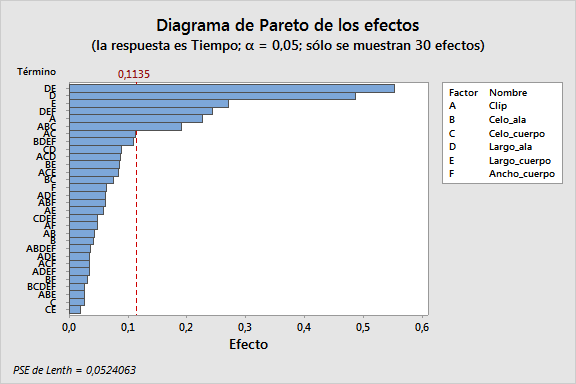
\includegraphics[width=0.45\linewidth]{imagenes/Experimento_fraccional/Pareto_de_los_efectos_para_Tiempo_(todos_los_factores)}}
	\subfigure[Gráfica de efectos normales]{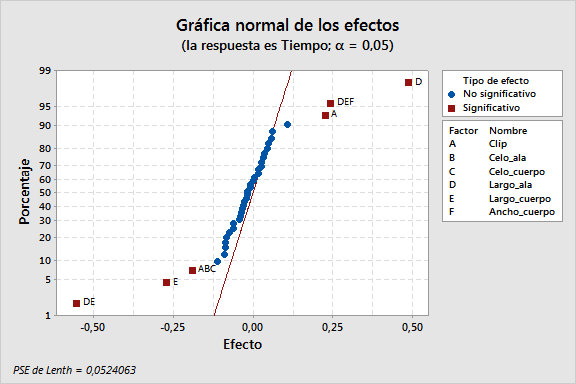
\includegraphics[width=0.45\linewidth]{imagenes/Experimento_fraccional/Grafica_de_los_efectos_para_Tiempo_(todos_los_factores)}}
	\caption{Resultado del modelo con todos los factores} \label{fig:resultado_experimento_fraccional_1}
\end{figure}

Observamos que los factores más significantes son el clip (A), el largo del ala (D) y el largo del cuerpo (E), junto con las interacciones del largo del ala y del cuerpo (DE), de los dos anteriores más el ancho del cuerpo (DEF), y la interacción entre el clip y los celos --ala y cuerpo-- (ABC).\\

Los efectos principales de este modelo se puede ver en la Figura~\ref{fig:efectos_principales_todos_los_factores}.\\

\begin{figure}[htbp!]
	\centering
	\subfigure[Gráfica de efectos principales]{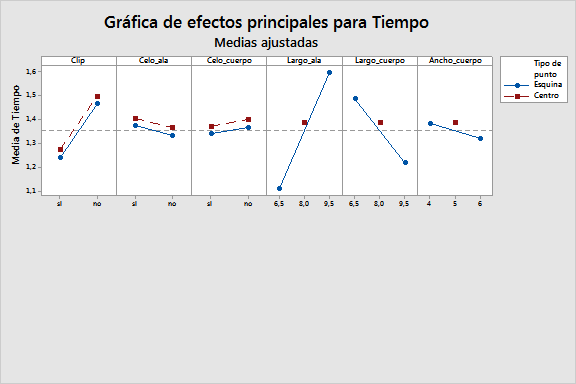
\includegraphics[width=0.45\linewidth]{imagenes/Experimento_fraccional/Grafica_de_efectos_principales_para_Tiempo_(todos_los_factores)}}
	\subfigure[Gráfica de interacción]{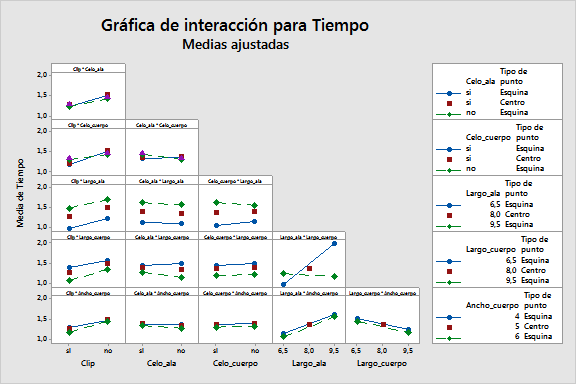
\includegraphics[width=0.45\linewidth]{imagenes/Experimento_fraccional/Grafica_de_interaccion_para_Tiempo_(todos_los_factores)}}
	\caption{Diagramas de efectos principales e interacción}
	\label{fig:efectos_principales_todos_los_factores}
\end{figure}

Se puede observar que los mayores efectos se producen en clip, largo ala y largo cuerpo. La mayor interacción se produce entre largo ala y largo cuerpo.\\

Con estos factores, procedemos a reducir el modelo, pero antes necesitamos comprobar si el modelo es adecuado. Para ello, representamos el diagrama de residuos, pero Minitab no nos lo muestra debido a la escasez de grados de libertad.\\

Reducimos el modelo con los factores A, D,E, DE, DEF, ABC. Minitab nos recomienda añadir al modelo otros factores como A, E, F y algunas interacciones. Los gráficos de Pareto y de efectos normales se muestran en la Figura~\ref{fig:resultado_experimento_fraccional_2}.\\

\begin{figure}[htbp!]
	\centering
	\subfigure[Gráfica de Pareto]{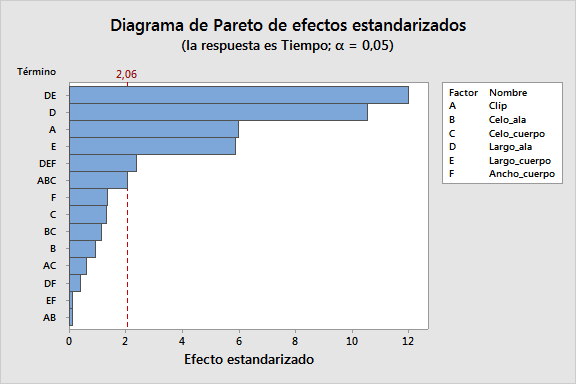
\includegraphics[width=0.45\linewidth]{imagenes/Experimento_fraccional/Pareto_de_los_efectos_para_Tiempo_2}}
	\subfigure[Gráfica de efectos normales]{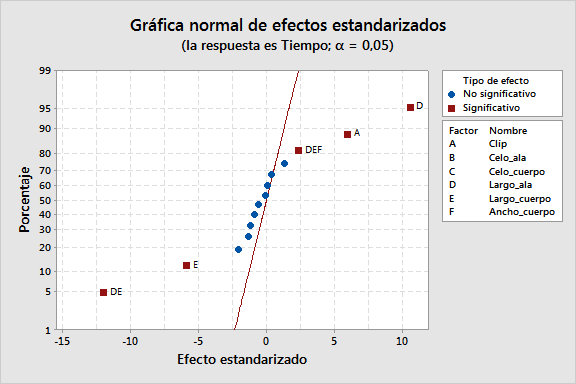
\includegraphics[width=0.45\linewidth]{imagenes/Experimento_fraccional/Grafica_de_los_efectos_para_Tiempo_2}}
	\caption{Resultado del modelo con todos los factores} \label{fig:resultado_experimento_fraccional_2}
\end{figure}

Se observa que ahora los factores más significativos son A, D, E y las interacciones DE y DEF.\\

Comprobemos el análisis de residuos de este modelo (Figura~\ref{fig:residuos_2}).\\

\begin{figure}[htbp!]
	\centering
	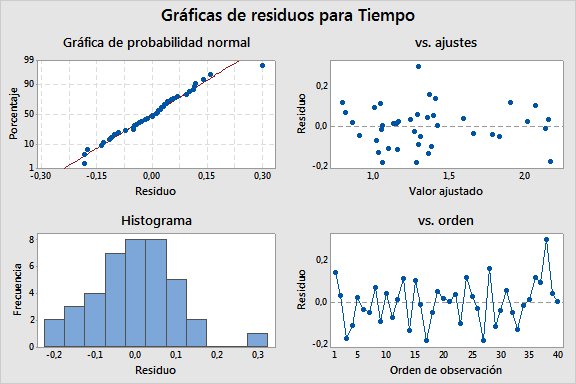
\includegraphics[width=0.7\linewidth]{imagenes/Experimento_fraccional/Graficas_de_residuos_para_Tiempo_2}
	\caption{Análisis de residuos para el segundo modelo}
	\label{fig:residuos_2}
\end{figure}

Nada parece indicar que se viola la normalidad, la aleatoriedad de los residuos o el orden de observación de los residuos.\\

Comprobamos si podemos simplificar el modelo de nuevo. Para ello, sólo añadimos al modelo los factores A, D, E y las interacciones DE y DEF. Los diagramas de Pareto y de interacción se muestran en la Figura~\ref{fig:resultado_experimento_fraccional_3}.\\

\begin{figure}[htbp!]
	\centering
	\subfigure[Gráfica de Pareto]{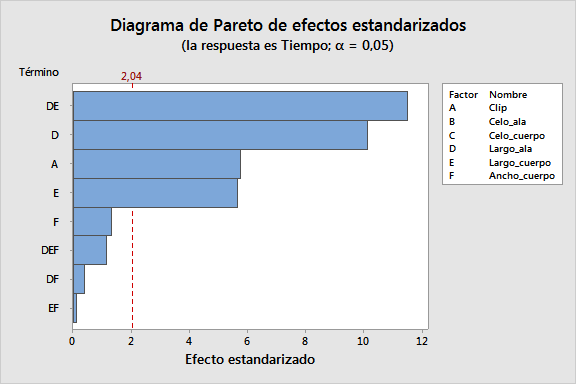
\includegraphics[width=0.45\linewidth]{imagenes/Experimento_fraccional/Pareto_de_los_efectos_para_Tiempo_3}}
	\subfigure[Gráfica de efectos normales]{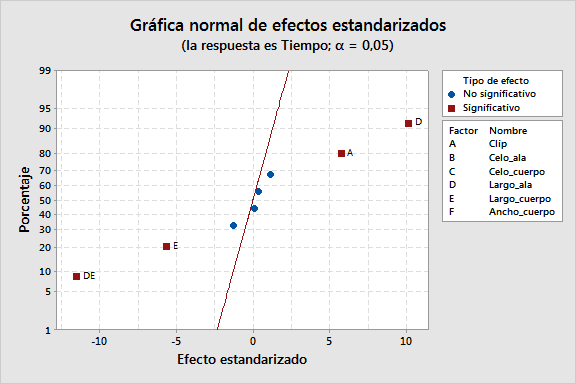
\includegraphics[width=0.45\linewidth]{imagenes/Experimento_fraccional/Grafica_de_los_efectos_para_Tiempo_3}}
	\caption{Resultado del modelo con todos los factores} \label{fig:resultado_experimento_fraccional_3}
\end{figure}

Observamos que las variables más significativas de este modelo son los factores A, D y E, y la interacción DE. Comprobamos las hipótesis de este modelo (Figura~\ref{fig:residuos_3}).\\

\begin{figure}[htbp!]
	\centering
	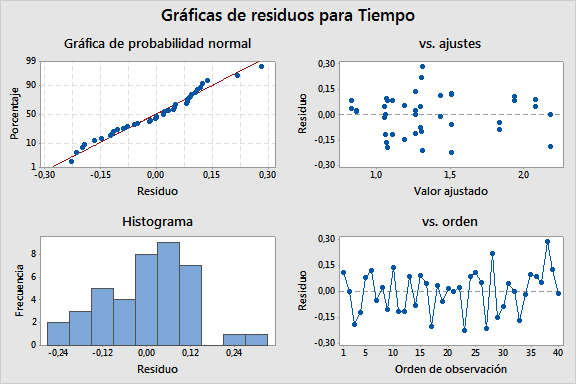
\includegraphics[width=0.7\linewidth]{imagenes/Experimento_fraccional/Graficas_de_residuos_para_Tiempo_3}
	\caption{Análisis de residuos para el tercer modelo}
	\label{fig:residuos_3}
\end{figure}

Nada parece indicar que no se cumplen las hipótesis de partida.\\

Para finalizar, simplificamos el modelo añadiendo sólo los factores A, D y E, y la interacción DE. Los gráficos de Pareto y de interacción de este modelo se puede ver en la Figura~\ref{fig:resultado_experimento_fraccional_4}.\\

\begin{figure}[htbp!]
	\centering
	\subfigure[Gráfica de Pareto]{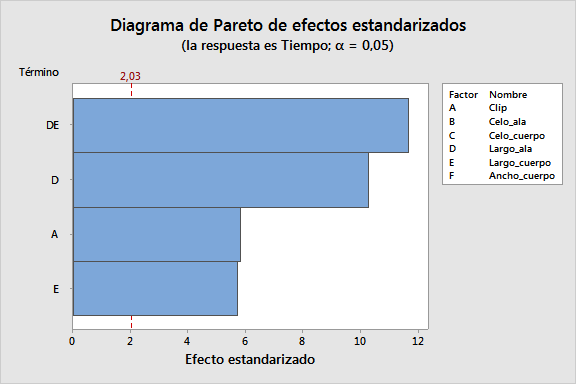
\includegraphics[width=0.45\linewidth]{imagenes/Experimento_fraccional/Pareto_de_los_efectos_para_Tiempo_4}}
	\subfigure[Gráfica de efectos normales]{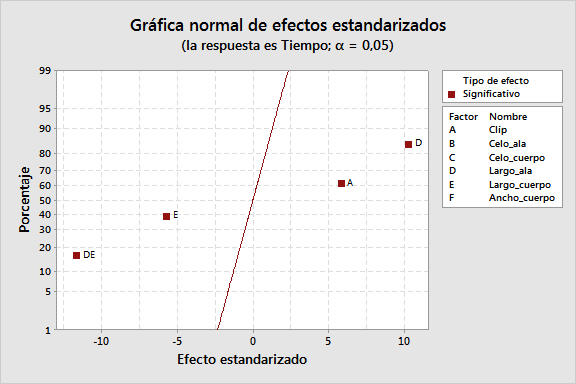
\includegraphics[width=0.45\linewidth]{imagenes/Experimento_fraccional/Grafica_de_los_efectos_para_Tiempo_4}}
	\caption{Resultado último del modelo} \label{fig:resultado_experimento_fraccional_4}
\end{figure}

Vemos que sólo quedan en el modelo variables significativas: A (clip), D (largo ala), E (largo cuerpo) y la interacción DE (interacción entre el largo del ala y del cuerpo).\\

La salida que devuelve Minitab es la siguiente:

\begin{verbatim}
Análisis de Varianza

Fuente                         GL  SC Ajust.  MC Ajust.  Valor F  Valor p
Modelo                          5    5,55313    1,11063    61,80    0,000
Lineal                        3    3,09826    1,03275    57,47    0,000
Clip                        1    0,60861    0,60861    33,87    0,000
Largo_ala                   1    1,90076    1,90076   105,77    0,000
Largo_cuerpo                1    0,58888    0,58888    32,77    0,000
Interacciones de 2 términos   1    2,44813    2,44813   136,22    0,000
Largo_ala*Largo_cuerpo      1    2,44813    2,44813   136,22    0,000
Curvatura                     1    0,00675    0,00675     0,38    0,544
Error                          34    0,61103    0,01797
Total                          39    6,16417


Resumen del modelo

R-cuad.  R-cuad.
S  R-cuad.  (ajustado)   (pred)
0,134058   90,09%      88,63%   86,28%


Coeficientes codificados

EE del
Término                  Efecto     Coef   coef.  Valor T  Valor p   VIF
Constante                         1,3542  0,0237    57,14    0,000
Clip                     0,2467   0,1233  0,0212     5,82    0,000  1,00
Largo_ala                0,4874   0,2437  0,0237    10,28    0,000  1,00
Largo_cuerpo            -0,2713  -0,1357  0,0237    -5,72    0,000  1,00
Largo_ala*Largo_cuerpo  -0,5532  -0,2766  0,0237   -11,67    0,000  1,00
Pt Ctral                          0,0325  0,0530     0,61    0,544  1,00


Ecuación de regresión en unidades no codificadas

Tiempo = -7,090 + 0,1233 Clip + 1,1459 Largo_ala + 0,8930 Largo_cuerpo
- 0,1229 Largo_ala*Largo_cuerpo + 0,0325 Pt Ctral


Ajustes y diagnósticos para observaciones poco comunes

                              Resid
Obs  Tiempo  Ajuste   Resid   est.
38  1,6000  1,3090  0,2910   2,35  R
\end{verbatim}

Vemos que estamos ante un método bastante bueno con un coeficiente de determinación ajustado de 0.8863. Vemos que todos los p-valores de los factores son menores que 0.05, salvo el punto central.\\

Así la ecuación del tiempo de vuelo en función de los demás factores viene dada por la siguiente ecuación:

\begin{multline*}
\text{Tiempo} = -7.090 + 0.1233 \text{Clip} + 1.1459 \text{Largo\_ala} + 0.8930 \text{Largo\_cuerpo} \\
- 0.1229 \text{Largo\_ala} \cdot \text{Largo\_cuerpo}
\end{multline*}

También, sólo se produce una observación poco común, la 38, con una predicción de 1.3090 y observado de 1.6000, una diferencia de 0.2910 segundos.\\

Calculamos los residuos del modelo para ver si se viola alguna de las hipótesis de partida (Figura~\ref{fig:residuos_4}).\\

\begin{figure}[htbp!]
	\centering
	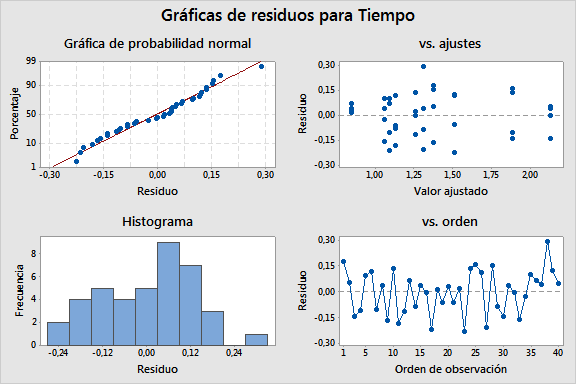
\includegraphics[width=0.7\linewidth]{imagenes/Experimento_fraccional/Graficas_de_residuos_para_Tiempo_4}
	\caption{Análisis de residuos para el último modelo}
	\label{fig:residuos_4}
\end{figure}

Parece que no se incumple ninguna de las hipótesis de partida.\\

Representamos la gráfica de cubo de este modelo (Figura~\ref{fig:cubo_fraccional}).\\

\begin{figure}[htbp!]
	\centering
	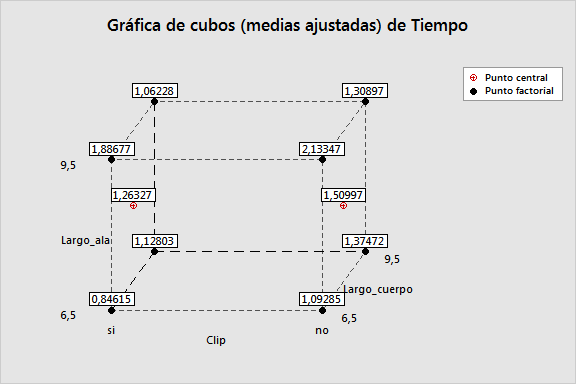
\includegraphics[width=0.7\linewidth]{imagenes/Experimento_fraccional/Grafica_de_cubos_(medias_ajustadas)_de_Tiempo_4}
	\caption{Gráfica de cubo}
	\label{fig:cubo_fraccional}
\end{figure}

El mayor tiempo de vuelo se consigue cuando no lleva clip, largo del ala de 9.5 cm y largo del cuerpo de 6.5 cm.\\

Para contrastar el modelo, añadimos una segunda mitad para respaldar lo obtenido con el apartado anterior, formando un experimento completo.  Los datos de este experimento se pueden encontrar en el Anexo~\ref{chp:experimentos}.\\

Comenzamos analizando el experimento, obteniéndose las gráficas de Pareto y de efectos normales (Figura~\ref{fig:resultado_experimento_completo_1}).\\

\begin{figure}[htbp!]
	\centering
	\subfigure[Gráfica de Pareto]{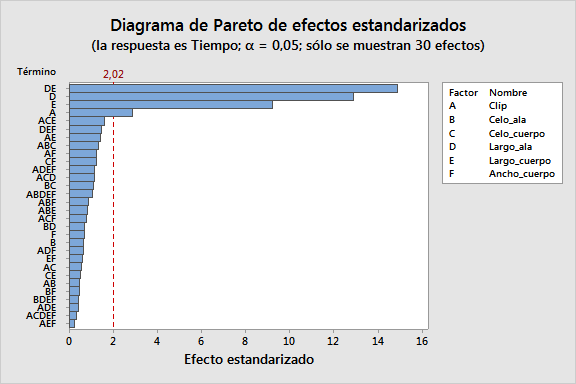
\includegraphics[width=0.45\linewidth]{imagenes/Experimento_completo/Pareto_de_los_efectos_para_Tiempo_1}}
	\subfigure[Gráfica de efectos normales]{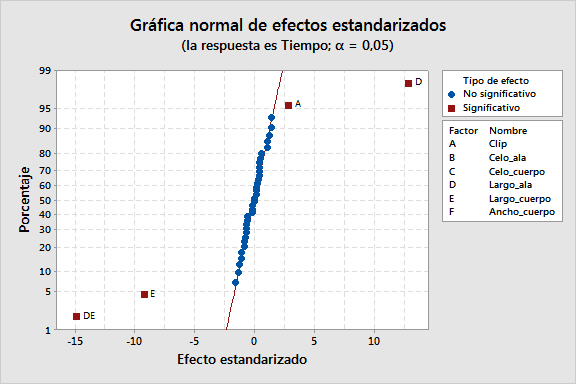
\includegraphics[width=0.45\linewidth]{imagenes/Experimento_completo/Grafica_de_los_efectos_para_Tiempo_1}}
	\caption{Resultados del experimento completo} \label{fig:resultado_experimento_completo_1}
\end{figure}

Los factores más significativos son A (clip), D (largo ala), E (largo cuerpo) y la interacción DE (largo del ala y del cuerpo).\\

Intentamos simplificar el modelo anterior añadiendo al modelo sólo los factores e interacciones significativas, esto es, A, D, E y DE.\\

Las gráficas de Pareto y de efectos normales de este nuevo modelo se pueden ver en la Figura~\ref{fig:resultado_experimento_completo_2}.\\

\begin{figure}[htbp!]
	\centering
	\subfigure[Gráfica de Pareto]{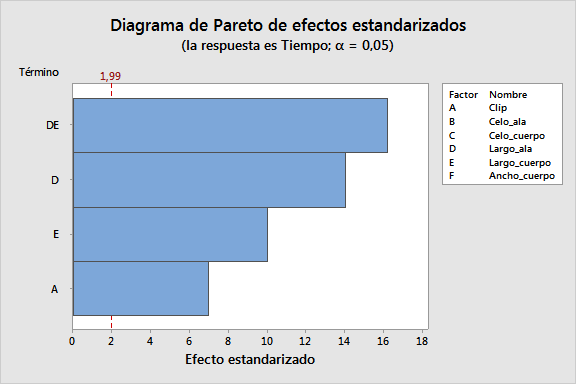
\includegraphics[width=0.45\linewidth]{imagenes/Experimento_completo/Pareto_de_los_efectos_para_Tiempo_2}}
	\subfigure[Gráfica de efectos normales]{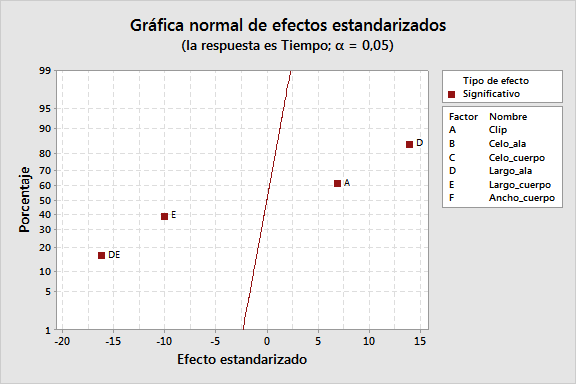
\includegraphics[width=0.45\linewidth]{imagenes/Experimento_completo/Grafica_de_los_efectos_para_Tiempo_2}}
	\caption{Resultados del experimento completo simplificado} \label{fig:resultado_experimento_completo_2}
\end{figure}

Vemos que todos los factores son significativos. Los resultados que devuelve Minitab son los siguientes:

\begin{verbatim}
Análisis de Varianza

Fuente                         GL  SC Ajust.  MC Ajust.  Valor F  Valor p
Modelo                          6    11,6635    1,94391   101,44    0,000
Bloques                         1     0,0314    0,03144     1,64    0,204
Lineal                          3     6,6107    2,20356   114,99    0,000
Clip                            1     0,9267    0,92665    48,36    0,000
Largo_ala                       1     3,7641    3,76409   196,42    0,000
Largo_cuerpo                    1     1,9200    1,91996   100,19    0,000
Interacciones de 2 términos     1     5,0204    5,02040   261,98    0,000
Largo_ala*Largo_cuerpo          1     5,0204    5,02040   261,98    0,000
Curvatura                       1     0,0009    0,00091     0,05    0,828
Error                          73     1,3989    0,01916
Total                          79    13,0624


Resumen del modelo

R-cuad.  R-cuad.
S  R-cuad.  (ajustado)   (pred)
0,138431   89,29%      88,41%   87,14%


Coeficientes codificados

EE del
Término                  Efecto     Coef   coef.  Valor T  Valor p   VIF
Constante                         1,3425  0,0173    77,58    0,000
Bloques
1                               0,0198  0,0155     1,28    0,204  1,00
Clip                     0,2152   0,1076  0,0155     6,95    0,000  1,00
Largo_ala                0,4850   0,2425  0,0173    14,02    0,000  1,00
Largo_cuerpo            -0,3464  -0,1732  0,0173   -10,01    0,000  1,00
Largo_ala*Largo_cuerpo  -0,5602  -0,2801  0,0173   -16,19    0,000  1,00
Pt Ctral                         -0,0085  0,0387    -0,22    0,828  1,00

Ecuación de regresión en unidades no codificadas

Tiempo = -6,994 + 0,1076 Clip + 1,1575 Largo_ala + 0,8804 Largo_cuerpo
- 0,12448 Largo_ala*Largo_cuerpo - 0,0085 Pt Ctral

Ecuación promediada sobre los bloques.

Ajustes y diagnósticos para observaciones poco comunes

                              Resid
Obs  Tiempo  Ajuste    Resid   est.
38  1,6000  1,2592   0,3408   2,58  R
47  1,0290  1,2947  -0,2657  -2,01  R
49  2,1870  1,9109   0,2761   2,09  R
67  1,1310  0,8657   0,2653   2,01  R

Residuo grande R
\end{verbatim}

Tenemos un modelo bastante bueno, con un ajuste de 0.8841, y todos los elementos del modelo tienen especial significación (p-valor < 0.05), excepto los puntos centrales, por lo que los descartamos.\\

La ecuación del modelo queda de la siguiente manera:

\begin{multline*}
\text{Tiempo} = -6.994 + 0.1076 \text{Clip} + 1.1575 \text{Largo\_ala} + 0.8804 \text{Largo\_cuerpo} - 0,12448 \text{Largo\_ala}\cdot \text{Largo\_cuerpo}
\end{multline*}

Para finalizar, representamos la gráfica de cubo de este modelo.\\

\begin{figure}[htbp!]
	\centering
	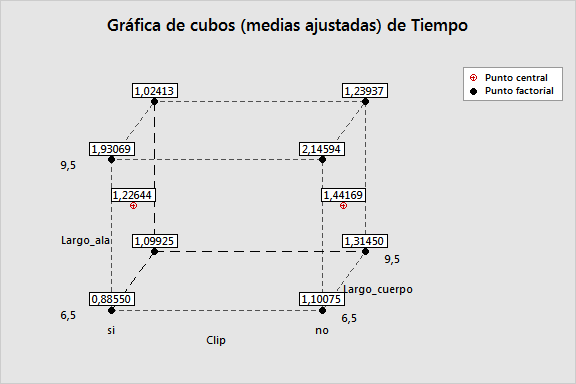
\includegraphics[width=0.7\linewidth]{imagenes/Experimento_completo/Grafica_de_cubos_(medias_ajustadas)_de_Tiempo}
	\caption{Gráfica de cubo del experimento completo}
	\label{fig:cubo_completo}
\end{figure}

El mayor tiempo de vuelo se consigue cuando no lleva clip, largo del ala de 9.5 cm y largo del cuerpo de 6.5 cm, con un tiempo de vuelo de 2.1459 segundos.\\

Con sendos experimentos, hemos obtenido un modelo de ajuste, bastante parecidos entre ellos. Parece ser que las variables clip, largo del ala y del cuerpo son variables influyentes en el tiempo de vuelo del helicóptero.

\subsection{Optimización del diseño y del proceso de fabricación}

Con todos los datos anteriores, ya estamos en disposición para mejorar el proceso. A tenor de los experimentos anteriores, las variables más influyentes para el tiempo de vuelo del helicóptero son el llevar o no clip, y el largo del ala y del cuerpo. Puesto que las demás variables no parecen tener demasiada influencia en el tiempo de vuelo, las ponemos al coste mínimo. Estas variables son celo del ala y del cuerpo que, a partir de ahora, nuestros helicópteros ya no llevarán (con su correspondiente ahorro), y el ancho del cuerpo que lo ponemos al mínimo de especificación (4 cm).\\

En torno al proceso, eliminamos la fase de pegado donde se pegaba con cinta adhesiva los bordes del cuerpo del helicóptero. Ya no es necesaria esta fase con el nuevo diseño. También eliminamos la fase de inspección, porque no aporta valor añadido al producto.\\

Por tanto, se debe realizar un reajuste en el reparto de los empleados en las diferentes tareas, quedando de la siguiente manera:

\begin{itemize}
	\item Etapa de corte: 3 personas más medio turno de otra
	\item Etapa de prueba de vuelo: 4 personas
	\item Etapa de etiquetado: 2 personas más medio turno de otra
\end{itemize}

\begin{table}[htbp!]
	\centering
	\caption{Número de unidades diarias por tareas (proceso mejorado)}
	\label{tbl:tiempos_finales}
	\begin{tabular}{@{}cccc@{}}
		\toprule
		Tarea        & \begin{tabular}[c]{@{}c@{}}Tiempo diario\\ (en horas)\end{tabular} & \begin{tabular}[c]{@{}c@{}}Tiempo en realizar tarea\\ por unidad (en segundos)\end{tabular} & \begin{tabular}[c]{@{}c@{}}Número de \\ unidades diarias\end{tabular} \\ \midrule
		Corte        & 28                                                                 & 55                                                                                          & 1\,832                                                                  \\
		Prueba vuelo & 32                                                                 & 55                                                                                          & 2\,094                                                                  \\
		Etiquetado   & 20                                                                 & 35                                                                                          & 2\,057                                                                  \\ \bottomrule
	\end{tabular}
\end{table}

Por tanto, la producción diaria teórica es de 1\,832 unidades. Si suponemos un rendimiento del 80\%, tenemos 1\,456 unidades fabricadas diariamente.\\

Mensualmente, tenemos una producción de 54\,960 unidades, lo que hacen unos ingresos totales de 329\,760 euros, a lo que hay que descontar los gastos fijos de los empleados y de mantenimiento, y los costes asociados a cada fase del proceso, tenemos un total de 255\,776 euros mensuales. Por tanto, el beneficio mensual de la empresa es de 73\,984 euros.\\

La Tabla~\ref{tbl:comparativa} muestra una comparativa de los costes y de la producción antes y después de aplicar la metodología Seis Sigma.\\

\begin{table}[htbp!]
	\centering
	\caption{Comparativa antes y después de Seis Sigma}
	\label{tbl:comparativa}
	\begin{tabular}{@{}ccc@{}}
		\cmidrule(l){2-3}
		& Antes             & Después          \\ \midrule
		Coste helicóptero  & 6 euros           & 6 euros          \\
		Producción diaria  & 987 unidades      & 1\,456 unidades  \\
		Producción mensual & 29\,616  unidades & 54\,960 unidades \\
		Ingresos mensuales & 117\,696 euros    & 329\,760 euros   \\
		Gastos mensuales   & 158\,445 euros    & 255\,776 euros   \\
		Beneficio mensual  & -40\,749 euros    & 73\,984 euros    \\ \bottomrule
	\end{tabular}
\end{table}

Por último, sólo nos queda calcular el diseño óptimo para lograr nuestro objetivo de lograr 1 de cada 2\,000 helicópteros que no cumplan el tiempo de vuelo especificado (> 1 segundo). Si lo calculamos sobre 1\,000\,000 de helicópteros deberíamos tener 500 que no lo cumplan. Es decir, nuestro proceso debería tener 4 sigmas para que esto se cumpliera \cite{Sigma}. Tomamos como desviación típica 0.4 del último experimento. Así el objetivo es 1+4*0.4 = 2.6 segundos.\\

Usando el optimizador de respuesta de Minitab, fijamos ese objetivos para obtener los valores de las variables óptimos para ese valor. Ejecutándolo nos devuelve que el tamaño óptimo es el de no usar clip, el largo del ala es de 9.5 cm y el largo del cuerpo es de 6.5 cm, logrando un tiempo de vuelo de 2.10 segundos. 
 

\section{Control}

Puesto que las variables que más afectan al tiempo de vuelo son la longitud de las alas y del cuerpo, debemos establecer métodos que nos permitan reducir la variabilidad del tiempo de vuelo de los helicópteros. Un método puede ser mejorar las herramientas de corte. Con unas herramientas más precisas se conseguirá que se reduzca al mínimo la cantidad de helicópteros defectuosos (tiempo de vuelo menor que 1 segundo) y mejorar la satisfacción del cliente, mejorando a su vez, la confianza depositada en Parasafe S.A. 

\section{Conclusiones}

Con la ayuda de la metodología Seis Sigma (DMAIC) hemos conseguido mejorar el proceso de fabricación y diseño de los helicópteros de papel. Empleando técnicas estadísticas clásicas bien conocidas como el diseño de experimentos, los contrastes de hipótesis o ANOVA se ha conseguido una mejora sustancial en el proceso, ahorrando una gran cantidad de dinero y tiempo.

%\bibliographystyle{plain}
%\bibliography{bibliografia}

\begin{appendices}
	\section{Datos de los experimentos} \label{chp:experimentos}
\end{appendices}



\end{document}